% !TeX root = ./0_Manuscript.tex

%%% Path
\RequirePackage{etoolbox}
\csdef{input@path}{%
 {sty/}% cls, sty files
 {img/}% eps files
 {bib/}% eps files
}%
\csgdef{bibdir}{bib/}% bst, bib files

\documentclass[11pt]{book}
\pdfoutput=1

%%% Styles
\usepackage{manuscriptLayout}
\usepackage{manuscriptCover}

\usepackage{amssymb,amsmath,amsthm,amsfonts}
%\usepackage[onelanguage,english,ruled,vlined,linesnumbered]{algorithm2e}
\usepackage{a4wide}
\usepackage{caption}
\usepackage{subcaption}
\usepackage{fancybox}
\usepackage{comment}% Diff
\usepackage{color}
%\usepackage{enumitem} % Pour changer le style des listes d'items
\usepackage[T1]{fontenc}
\usepackage{graphicx}
\usepackage{geometry}
\usepackage{tocloft}
\usepackage[tight]{minitoc}
\usepackage{natbib}
% \usepackage{bibtex}
% \usepackage{biblatex}
\usepackage{palatino}
\usepackage{placeins}
\usepackage{pgf}
\usepackage{subfloat}
%\usepackage{subfig}
\usepackage{tabularx}
\usepackage{tikz}
\usepackage[european, noarrowmos]{circuitikz}
\usepackage{svg}
\usepackage{import}
%\usepackage[linesnumbered,ruled,vlined]{algorithm2e}
\usepackage{algorithm}
%\usepackage{algorithmic}
\usepackage{algpseudocode}
\usepackage{glossaries}
\usepackage{fancyvrb}
%\usepackage[filename=0_Manuscript, mouseover, movetips, inactive]{fancytooltips}

\usepackage{hyperref}

\usepackage{datetime2}
\usepackage{textgreek}
\usepackage{textcomp}
%\usepackage{layouts}
\usepackage[export]{adjustbox}
%\usepackage[dvipsnames]{xcolor}
\usepackage{colortbl}
\usepackage{hhline}
\usepackage{tabu}
\usepackage{tabularx}
\usepackage{bibentry}
\usepackage{csquotes}
\usepackage{xspace}
%\showboxes
%\showframe

\definecolor{myCyan}{RGB}{59, 204, 255}
\definecolor{myViolet}{RGB}{169, 0, 173}
\newcommand{\cRef}[2]{\hyperref[#1]{\textcolor{myViolet}{#2}}}
\newcommand{\fiftyOhms}[1]{\mbox{#1 \textOmega\xspace}}
\newcommand{\cGood}{\rowcolor{green!25}}
\newcommand{\cOk}{\rowcolor{blue!25}}
\newcommand{\cBad}{\rowcolor{orange!25}}
\newcommand{\cErr}{\rowcolor{red!25}}
\newcommand{\cYe}{\rowcolor{yellow!25}}


%%%%%%%%%%%%%%%%%%%%%%%%%%%%%%----------------------%%%%%%%%%%%%%%%%%%%%%%%%%%%%%%%%%%

%% Comment the three (or more) next lines that ar not already commented before compiling final build %%
%\usepackage[inline]{showlabels}
%\newcommand{\DDC}{\textcolor{myCyan}{\footnotesize COMPILATION DATE: \DTMnow}}
%\newcommand{\ddc}{\textcolor{myCyan}{\footnotesize COMPILATION DATE: \DTMnow}}
\newcommand{\DDC}{\textcolor{myCyan}{\footnotesize \DTMnow}}
\newcommand{\ddc}{\textcolor{myCyan}{\footnotesize \DTMnow}}

%% Uncomment the three next lines before compiling final build %%
%\usepackage[final]{showlabels}
%\newcommand{\DDC}{}
%\newcommand{\ddc}{}

%%%%%%%%%%%%%%%%%%%%%%%%%%%%%%----------------------%%%%%%%%%%%%%%%%%%%%%%%%%%%%%%%%%%

%custom adac

%\usepackage[export]{adjustbox}
%\usepackage[all]{hypcap}
%\usepackage{textcomp, textgreek}
%\usepackage{color, soul}
%\usepackage{booktabs}
%\usepackage{array}
%\usepackage{multirow}
%\usepackage{makecell}
%\usepackage[newfloat]{minted}
%\usepackage{xfrac}

%\usepackage[nottoc]{tocbibind}
%\usepackage{etoolbox}

\usetikzlibrary{
    positioning,
    backgrounds,
    shapes,
    arrows.meta,
    calc
}

%\usepackage{subcaption}

%\usepackage{yhmath}

%\SetKwInput{KwInput}{Entrées}                % Set the Input
%\SetKwInput{KwOutput}{Sorties}              % set the Output
%\SetKwInput{KwInit}{Initialisations}


%%% Options packages
%\frenchbsetup{StandardLists=true}
\selectcolormodel{RGB}
\geometry{%
  a4paper, %body={150mm,220mm},
  left=25mm,top=30mm,
  headheight=7mm,
  headsep=14mm,
  marginparsep=4mm, marginparwidth=27mm
}

\setstretch{1.25}

\setcounter{minitocdepth}{2}
\setcounter{tocdepth}{2}
\setcounter{secnumdepth}{4}

%\makeatletter
%\pretocmd{\chapter}{\addtocontents{toc}{\protect\addvspace{-5\p@}}}{}{}
%\pretocmd{\section}{\addtocontents{toc}{\protect\addvspace{-10\p@}}}{}{}
%\pretocmd{\subsection}{\addtocontents{toc}{\protect\addvspace{-10\p@}}}{}{}
%%\pretocmd{\figure}{\addtocontents{tof}{\protect\addvspace{-10\p@}}}{}{}
%\makeatother

%\renewcommand\cftbeforechapskip{\vskip7pt}
%\renewcommand\cftbeforesecskip{\vskip5pt}
%\renewcommand\cftbeforefigskip{\vskip5pt}
%\renewcommand\cftchapafterpnum{\vskip5pt}
%\renewcommand\cftsecafterpnum{\vskip7pt}
%\renewcommand\cftsubsecafterpnum{\vskip2pt}
%\renewcommand\cftfigafterpnum{\vskip5pt}
%\renewcommand\cfttabafterpnum{\vskip5pt}

% ============================================================================
% Custom commands

% !TeX root = ./0_Manuscript.tex

\tikzset{
    fc-term/.style={ draw, align=center, rounded rectangle },
    fc-proc/.style={ draw, align=center, rectangle },
    fc-dec/.style={ draw, align=center, diamond, aspect=1.65 },
    %fc-subproc/.style={ draw, rectangle },
    fc-loop-start/.style={ draw, align=center, signal, signal to=south },
    fc-loop-end/.style={ draw, align=center, signal, signal to=north },
    fc-yes/.style={-latex},
    fc-no/.style={{Circle[open, length=5pt]}-latex}
}

\newcommand{\tochap}[1]{\hyperref[#1]{Chapter~\ref{#1}}}
\newcommand{\tosec}[1]{\hyperref[#1]{Section~\ref{#1}}}
\newcommand{\totab}[1]{\hyperref[#1]{Table~\ref{#1}}}
\newcommand{\tofig}[1]{\hyperref[#1]{Figure~\ref{#1}}}
\newcommand{\tofigs}[0]{Figures~}

\newcommand{\todo}[1]{{\color{red}\textbf{[TODO: #1]}}}
\newcommand*\circled[1]{\tikz[baseline=(char.base)]{
            \node[shape=circle,draw,inner sep=1pt] (char) {#1};}}
\newcommand*\fillcircled[1]{\tikz[baseline=(char.base)]{
            \node[shape=circle, fill=black, text=white, draw=black, inner sep=0.1em] (char) {#1};}}

\newcommand\Tstrut{\rule{0pt}{2.6ex}}       % "top" strut
\newcommand\Bstrut{\rule[-0.9ex]{0pt}{0pt}} % "bottom" strut
\newcommand{\TBstrut}{\Tstrut\Bstrut}       % top&bottom struts

\DeclareUnicodeCharacter{24EA}{\circled{0}}
\DeclareUnicodeCharacter{2460}{\circled{1}}
\DeclareUnicodeCharacter{2461}{\circled{2}}
\DeclareUnicodeCharacter{2462}{\circled{3}}
\DeclareUnicodeCharacter{2463}{\circled{4}}
\DeclareUnicodeCharacter{2464}{\circled{5}}
\DeclareUnicodeCharacter{2465}{\circled{6}}
\DeclareUnicodeCharacter{2466}{\circled{7}}
\DeclareUnicodeCharacter{2467}{\circled{8}}
\DeclareUnicodeCharacter{2468}{\circled{9}}
\DeclareUnicodeCharacter{24B6}{\circled{A}}
\DeclareUnicodeCharacter{24B7}{\circled{B}}
\DeclareUnicodeCharacter{24B8}{\circled{C}}
\DeclareUnicodeCharacter{24B9}{\circled{D}}
\DeclareUnicodeCharacter{24BA}{\circled{E}}
\DeclareUnicodeCharacter{24BB}{\circled{F}}

\DeclareUnicodeCharacter{24FF}{\fillcircled{0}}
\DeclareUnicodeCharacter{2776}{\fillcircled{1}}
\DeclareUnicodeCharacter{2777}{\fillcircled{2}}
\DeclareUnicodeCharacter{2778}{\fillcircled{3}}
\DeclareUnicodeCharacter{2779}{\fillcircled{4}}
\DeclareUnicodeCharacter{2780}{\fillcircled{5}}
\DeclareUnicodeCharacter{2781}{\fillcircled{6}}
\DeclareUnicodeCharacter{2782}{\fillcircled{7}}
\DeclareUnicodeCharacter{2783}{\fillcircled{8}}
\DeclareUnicodeCharacter{2784}{\fillcircled{9}}
\DeclareUnicodeCharacter{215}{\ensuremath{\times}}
\DeclareUnicodeCharacter{2192}{\ensuremath{\rightarrow}}
\DeclareUnicodeCharacter{394}{\ensuremath{\Delta}}

\newcommand*\floor[1]{\left\lfloor{#1}\right\rfloor}
\newcommand*\ceil[1]{\left\lceil{#1}\right\rceil}

\newcommand*{\Vdd}{\ensuremath{V_{DD}}\xspace}
\newcommand*{\GND}{\ensuremath{GND}\xspace}
\newcommand*{\halfVdd}{\ensuremath{\frac{1}{2}\Vdd}\xspace}
\newcommand*{\tRC}{\ensuremath{t_{RC}}\xspace}
\newcommand*{\tREFW}{\ensuremath{t_{REFW}}\xspace}
\newcommand*{\tREFI}{\ensuremath{t_{REFI}}\xspace}
\newcommand*{\tRFC}{\ensuremath{t_{RFC}}\xspace}
\newcommand*{\tRRDS}{\ensuremath{t_{RRD\_S}}\xspace}
\newcommand*{\tRRDL}{\ensuremath{t_{RRD\_L}}\xspace}
\newcommand*{\tFAW}{\ensuremath{t_{FAW}}\xspace}
\newcommand*{\TRH}{\ensuremath{T_{RH}}\xspace}
\newcommand*{\Nbank}{\ensuremath{N_{bank}}\xspace}
\newcommand*{\HCfirst}{\ensuremath{HC_{first}}\xspace}
\newcommand*{\ie}{\textit{i.e.}\xspace}
\newcommand*{\eg}{\textit{e.g.}\xspace}
\newcommand*{\electron}{{\fontsize{3pt}{3pt} \textbf{\fillcircled{$-$}}}}
\newcommand*{\bigElectron}{{\small \textbf{\fillcircled{$-$}}}}

\newcommand*{\hex}[1]{\ensuremath{\text{\texttt{#1}}_\text{h}}\xspace}
\newcommand*{\bin}[1]{\ensuremath{\text{\texttt{#1}}_\text{2}}\xspace}


\newcommand{\PreserveBackslash}[1]{\let\temp=\\#1\let\\=\temp}
\newcolumntype{C}[1]{>{\PreserveBackslash\centering}p{#1}}
\newcolumntype{R}[1]{>{\PreserveBackslash\raggedleft}p{#1}}
\newcolumntype{L}[1]{>{\PreserveBackslash\raggedright}p{#1}}

\newcommand{\latexComment}[1]{}

\newcommand{\head}[1]{{\noindent\textbf{#1.}\xspace}} % for heading of a paragraph

\newcommand\mycommfont[1]{\small\textcolor{blue}{#1}}
%\SetCommentSty{mycommfont}


\hyphenation{
    aca-demia
    Row-hammer
    Program-mable
}

\newenvironment{vcenterpage}
{\newpage\vspace*{\fill}\thispagestyle{empty}\renewcommand{\headrulewidth}{0pt}}
{\vspace*{\fill}}
%\endlocaldefs

\pagestyle{fancy}
\makeatletter
\DeclareRobustCommand{\format@sec@number}[2]{{\normalfont\upshape#1}#2}
\renewcommand{\chaptermark}[1]{%
  \markboth{\format@sec@number{\ifnum\c@secnumdepth>\m@ne\@chapapp\ \thechapter. \fi}{#1}}{}}
\renewcommand{\sectionmark}[1]{%
  \markright{\format@sec@number{\ifnum\c@secnumdepth>\z@\thesection. \fi}{#1}}}
\makeatother

\fancyhf{}
\fancyhead[RE]{\itshape\nouppercase{\leftmark}}
\fancyhead[LO]{\itshape\nouppercase{\rightmark}}
\fancyhead[LE,RO]{\thepage}

\fancypagestyle{default}{%
    \fancyhead[RE]{\itshape\nouppercase{\leftmark}}
    \fancyhead[LO]{\itshape\nouppercase{\rightmark}}
    \fancyhead[LE,RO]{\thepage}
}

\fancypagestyle{listofacronyms}{%
    \fancyhead[RE]{\itshape\nouppercase{List of Acronyms}}
    \fancyhead[LO]{\itshape\nouppercase{\rightmark}}
    \fancyhead[LE,RO]{\thepage}
}%

%\addto\captionsfrench{
%    \renewcommand{\mtctitle}{Table of content}
%    \renewcommand{\listfigurename}{List of the Figures}
%    \renewcommand{\listalgorithmcfname}{List of the Algorithms}
%}

%%%%%%%%%%%%%%%%%%%%%%%%%%%%%%%%%%%%%%%%%%%%%%%%%%%%%%%%%%%%%%%%%%%%%%%%%%%%%%%%%%
\usepackage{pdfbase}[2017/03/16]
\usepackage{xparse,ocgbase}
\usepackage{xcolor,calc}
\usepackage{tikzpagenodes,linegoal}
\usetikzlibrary{calc}
\usepackage{tcolorbox}

\ExplSyntaxOn
\let\tpPdfLink\pbs_pdflink:nn
\let\tpPdfAnnot\pbs_pdfannot:nnnn\let\tpPdfLastAnn\pbs_pdflastann:
\let\tpAppendToFields\pbs_appendtofields:n
\def\tpPdfXform{\pbs_pdfxform:nnnnn{1}{1}{}{}}
\let\tpPdfLastXform\pbs_pdflastxform:
\let\cListSet\clist_set:Nn\let\cListItem\clist_item:Nn
\ExplSyntaxOff

\makeatletter
\NewDocumentCommand{\tooltip}{%
    ssssO{\ifdefined\@linkcolor\@linkcolor\else blue\fi}mO{yellow!20}mO{0pt,0pt}%
}{{%
        \leavevmode%
        \IfBooleanT{#2}{%
            %for variants with two and more stars, put tip box on a PDF Layer (OCG)
            \ocgbase@new@ocg{tipOCG.\thetcnt}{%
                /Print<</PrintState/OFF>>/Export<</ExportState/OFF>>%
            }{false}%
            \xdef\tpTipOcg{\ocgbase@last@ocg}%
            %prevent simultaneous visibility of multiple non-draggable tooltips
            \ocgbase@add@ocg@to@radiobtn@grp{tool@tips}{\ocgbase@last@ocg}%
        }%
        \tpPdfLink{%
            \IfBooleanTF{#4}{%
                /Subtype/Link/Border[0 0 0]/A <</S/SetOCGState/State [/Toggle \tpTipOcg]>>
            }{%
                /Subtype/Screen%
                /AA<<%
                \IfBooleanTF{#3}{%
                    /E<</S/SetOCGState/State [/Toggle \tpTipOcg]>>%
                }{%
                    \IfBooleanTF{#2}{%
                        /E<</S/SetOCGState/State [/ON \tpTipOcg]>>%
                        /X<</S/SetOCGState/State [/OFF \tpTipOcg]>>%
                    }{
                        \IfBooleanTF{#1}{%
                            /E<</S/JavaScript/JS(%
                            var fd=this.getField('tip.\thetcnt');%
                            if(typeof(click\thetcnt)=='undefined'){%
                                var click\thetcnt=false;%
                                var fdor\thetcnt=fd.rect;var dragging\thetcnt=false;%
                            }%
                            if(fd.display==display.hidden){%
                                fd.delay=true;fd.display=display.visible;fd.delay=false;%
                            }else{%
                                if(!click\thetcnt&&!dragging\thetcnt){fd.display=display.hidden;}%
                                if(!dragging\thetcnt){click\thetcnt=false;}%
                            }%
                            this.dirty=false;%
                            )>>%
                        }{%
                            /E<</S/JavaScript/JS(%
                            var fd=this.getField('tip.\thetcnt');%
                            if(typeof(click\thetcnt)=='undefined'){%
                                var click\thetcnt=false;%
                                var fdor\thetcnt=fd.rect;var dragging\thetcnt=false;%
                            }%
                            if(fd.display==display.hidden){%
                                fd.delay=true;fd.display=display.visible;fd.delay=false;%
                            }%
                            this.dirty=false;%
                            )>>%
                            /X<</S/JavaScript/JS(%
                            if(!click\thetcnt&&!dragging\thetcnt){fd.display=display.hidden;}%
                            if(!dragging\thetcnt){click\thetcnt=false;}%
                            this.dirty=false;%
                            )>>%
                        }%
                        /U<</S/JavaScript/JS(click\thetcnt=true;this.dirty=false;)>>%
                        /PC<</S/JavaScript/JS (%
                        var fd=this.getField('tip.\thetcnt');%
                        try{fd.rect=fdor\thetcnt;}catch(e){}%
                        fd.display=display.hidden;this.dirty=false;%
                        )>>%
                        /PO<</S/JavaScript/JS(this.dirty=false;)>>%
                    }%
                }%
                >>%
            }%
        }{{\color{#5}#6}}%
        \sbox\tiptext{%
            \IfBooleanT{#2}{%
                \ocgbase@oc@bdc{\tpTipOcg}\ocgbase@open@stack@push{\tpTipOcg}}%
            %\fcolorbox{black}{#7}{#8}%
            \tcbox[colframe=black,colback=#7,size=fbox,arc=1ex,sharp corners=southwest]{#8}%
            \IfBooleanT{#2}{\ocgbase@oc@emc\ocgbase@open@stack@pop\tpNull}%
        }%
        \cListSet\tpOffsets{#9}%
        \edef\twd{\the\wd\tiptext}%
        \edef\tht{\the\ht\tiptext}%
        \edef\tdp{\the\dp\tiptext}%
        \tipshift=0pt%
        \IfBooleanTF{#2}{%
            %OCG-based (that is, all non-draggable) boxes should not extend beyond the
            %current column as they may get overlaid by text in the neighbouring column
            \setlength\whatsleft{\linegoal}%
        }{%
            \measureremainder{\whatsleft}%
        }%
        \ifdim\whatsleft<\dimexpr\twd+\cListItem\tpOffsets{1}\relax%
        \setlength\tipshift{\whatsleft-\twd-\cListItem\tpOffsets{1}}\fi%
        \IfBooleanF{#2}{\tpPdfXform{\tiptext}}%
        \raisebox{\heightof{#6}+\tdp+\cListItem\tpOffsets{2}}[0pt][0pt]{%
            \makebox[0pt][l]{\hspace{\dimexpr\tipshift+\cListItem\tpOffsets{1}\relax}%
                \IfBooleanTF{#2}{\usebox{\tiptext}}{%
                    \tpPdfAnnot{\twd}{\tht}{\tdp}{%
                        /Subtype/Widget/FT/Btn/T (tip.\thetcnt)%
                        /AP<</N \tpPdfLastXform>>%
                        /MK<</TP 1/I \tpPdfLastXform/IF<</S/A/FB true/A [0.0 0.0]>>>>%
                        /Ff 65536/F 3%
                        /AA <<%
                        /U <<%
                        /S/JavaScript/JS(%
                        var fd=event.target;%
                        var mX=this.mouseX;var mY=this.mouseY;%
                        var drag=function(){%
                            var nX=this.mouseX;var nY=this.mouseY;%
                            var dX=nX-mX;var dY=nY-mY;%
                            var fdr=fd.rect;%
                            fdr[0]+=dX;fdr[1]+=dY;fdr[2]+=dX;fdr[3]+=dY;%
                            fd.rect=fdr;mX=nX;mY=nY;%
                        };%
                        if(!dragging\thetcnt){%
                            dragging\thetcnt=true;Int=app.setInterval("drag()",1);%
                        }%
                        else{app.clearInterval(Int);dragging\thetcnt=false;}%
                        this.dirty=false;%
                        )%
                        >>%
                        >>%
                    }%
                    \tpAppendToFields{\tpPdfLastAnn}%
                }%
        }}%
        \stepcounter{tcnt}%
}}
\makeatother
\newsavebox\tiptext\newcounter{tcnt}
\newlength{\whatsleft}\newlength{\tipshift}
\newcommand{\measureremainder}[1]{%
    \begin{tikzpicture}[overlay,remember picture]
        \path let \p0 = (0,0), \p1 = (current page.east) in
        [/utils/exec={\pgfmathsetlength#1{\x1-\x0}\global#1=#1}];
    \end{tikzpicture}%
}
%%%%%%%%%%%%%%%%%%%%%%%%%%%%%%%%%%%%%%%%%%%%%%%%%%%%%%%%%%%%%%%%%%%%%%%%%%%%%%%%%%

%\mtcsetoffset{minitoc}{-10cm}
%\nomtcrule

%\titlespacing{\chapter}{0cm}{0cm}{-10cm}
%\chapterbelowskip{\vspace*{2cm}}

\newcommand{\twF}{Triple-Well\xspace}
\newcommand{\dwF}{Dual-Well\xspace}

\newcommand{\aes}{\tooltip[black]{AES}[orange]{Advanced Envryption Standard}\xspace}
\newcommand{\bbi}{\tooltip[black]{BBI}[orange]{Body Biasing Injection}\xspace}
\newcommand{\bsim}{\tooltip[black]{BSIM}[orange]{Berkeley Short-channel IGFET Model}\xspace}
\newcommand{\cps}{\tooltip[black]{CPS}[orange]{Cyber-Physical System}\xspace}
\newcommand{\des}{\tooltip[black]{DES}[orange]{Data Encryption Standard}\xspace}
\newcommand{\dom}{\tooltip[black]{DoM}[orange]{Difference of Means}\xspace}
\newcommand{\dfa}{\tooltip[black]{DFA}[orange]{Differential Fault Analysis}\xspace}
\newcommand{\dpa}{\tooltip[black]{DPA}[orange]{Differential Power Analysis}\xspace}
\newcommand{\dw}{\tooltip[black]{DW}[orange]{Dual-Well}\xspace}
\newcommand{\ecc}{\tooltip[black]{ECC}[orange]{Elliptic-Curve Cryptography}\xspace}
\newcommand{\esd}{\tooltip[black]{ESD}[orange]{Electrostatic Discharge}\xspace}
\newcommand{\emfi}{\tooltip[black]{EMFI}[orange]{Electromagnetic Fault Injection}\xspace}
\newcommand{\gcfam}{\tooltip[black]{FAM}[orange]{Fault Analysis Mapping}\xspace}
\newcommand{\fib}{\tooltip[black]{FIB}[orange]{Focused Ion Beam}\xspace}
\newcommand{\fsa}{\tooltip[black]{FSA}[orange]{Fault Sensibility Analysis}\xspace}
\newcommand{\fsm}{\tooltip[black]{FSM}[orange]{Fault Susceptibility Map}\xspace}
\newcommand{\gfi}{\tooltip[black]{GFI}[orange]{Glitch Fault Injection}\xspace}

\newcommand{\hfi}{\tooltip[black]{HFI}[orange]{Hardware Fault Injection}\xspace}
\newcommand{\ic}{\tooltip[black]{IC}[orange]{Integrated Circuit}\xspace}
\newcommand{\iot}{\tooltip[black]{IoT}[orange]{Internet of Things}\xspace}
\newcommand{\lfi}{\tooltip[black]{LFI}[orange]{Laser Fault Injection}\xspace}
\newcommand{\pcc}{\tooltip[black]{PCC}[orange]{Pearson Correlation Coefficient}\xspace}
\newcommand{\pll}{\tooltip[black]{PLL}[orange]{Phase Locked Loop}\xspace}
\newcommand{\ram}{\tooltip[black]{RAM}[orange]{Random Access Memory}\xspace}
\newcommand{\rsa}{\tooltip[black]{RSA}[orange]{Rivest–Shamir–Adleman}\xspace}
\newcommand{\sca}{\tooltip[black]{SCA}[orange]{Side Channel Attack/Analysis}\xspace}
\newcommand{\scs}{\tooltip[black]{SCS}[orange]{Standard-Cell Segment}\xspace}
\newcommand{\sma}{\tooltip[black]{SCS}[orange]{SubMiniature version A}\xspace}
\newcommand{\spa}{\tooltip[black]{SPA}[orange]{Simple Power Analysis}\xspace}
\newcommand{\tw}{\tooltip[black]{TW}[orange]{Triple-Well}\xspace}
\newcommand{\wlcsp}{\tooltip[black]{WLCSP}[orange]{Wafer-Level Chip-Scale Packaging}\xspace}

\pdfminorversion=5
\pdfcompresslevel=9
\pdfobjcompresslevel=2

\parskip 0.4cm
\begin{document}
%\pagenumbering{roman}
%\NoAutoSpacing
\frontmatter

\title{\protect\parbox{\textwidth}{\protect\centering Body biasing fault injection: modeling}}
\author{Geoffrey Chancel}

\directorA{TO BE COMPLETED}
%\directorB{TO BE COMPLETED}

\date{COMPILATION DATE: \DDC}

\thispagestyle{empty}

\university{UNIVERSITY OF MONTPELLIER}
\univlogo{logo_um_2020_rouge_CMJN.pdf}
\univwallpaper{logo_um_these_back.pdf}
\doctoral{Information, Structures, and Systems sciences}
\researchunit{LIRMM}
\specialisation{SyAM - Automatic and Microelectronic Systems}
\jury{Philippe Maurine  }{ Associate Professor ?? }{ University of Montpellier }{ Thesis Director    }
\jury{Jean-Marc Gallière}{ Associate Professor ?? }{ University of Montpellier }{ Thesis Supervisor }

\maketitle

\cleardoublepage
% !TeX root = ./0_Manuscript.tex

\section*{Abstract \DDC}

\section*{Résumé de la thèse \DDC}

% !TeX root = ./0_Manuscript.tex

\section*{Acknowledgements \DDC}

\textit{The authors acknowledge the support of the French Agence Nationale de la Recherche (ANR), under grant ANR-19-CE39-0008 (project ARCHI-SEC).
They also acknowledge the French Ministère des Armées -- Agence de l’innovation de défense (AID) under grant ID-UM-2019 65 0036.}

\adjustmtc
\dominitoc

\cleardoublepage
\tableofcontents

\cleardoublepage
\phantomsection
\addcontentsline{toc}{chapter}{\listfigurename}
\listoffigures
\mtcaddchapter

\cleardoublepage
\phantomsection
\addcontentsline{toc}{chapter}{\listtablename}
\listoftables
\mtcaddchapter

\cleardoublepage
\phantomsection
%\addcontentsline{toc}{chapter}{\listalgorithmcfname}
\addcontentsline{toc}{chapter}{List of algorithms}
\mtcaddchapter
\listofalgorithms

\cleardoublepage
\phantomsection
\thispagestyle{empty}
\addcontentsline{toc}{chapter}{List of acronyms}
\mtcaddchapter

% !TeX root = ./0_Manuscript.tex

\vspace*{60pt}
\textbf{\Huge List of Acronyms}
\vspace{25pt}
\pagestyle{listofacronyms}

\begin{tabular}{p{2.5cm}l}
    \textbf{BBI}        & \textbf{B}ody \textbf{B}iasing \textbf{I}njection \\
    \textbf{BSIM}        & \textbf{B}erkeley \textbf{S}hort-channel \textbf{I}GFET \textbf{M}odel \\
    \textbf{DPA}        & \textbf{D}ifferential \textbf{P}ower \textbf{A}nalysis \\
    \textbf{ECC}        & \textbf{E}lliptic-\textbf{C}urve \textbf{C}ryptography \\
    \textbf{EMFI}        & \textbf{E}lectro-\textbf{M}agnetic \textbf{F}ault \textbf{I}njection \\
    \textbf{FAM}        & \textbf{F}ault \textbf{A}nalysis \textbf{M}apping \\
    \textbf{FIB}        & \textbf{F}ocused \textbf{I}on \textbf{B}eam \\
    \textbf{FSM}        & \textbf{F}ault \textbf{S}usceptibility \textbf{M}ap \\
    \textbf{LFI}        & \textbf{L}aser \textbf{F}ault \textbf{I}njection \\
    \textbf{RAM}        & \textbf{R}andom \textbf{A}ccess \textbf{M}emory\\
    \textbf{SCA}        & \textbf{S}ide \textbf{C}hannel \textbf{A}ttack\\
\end{tabular}

\begin{tabular}{p{2.5cm}l}
    \textbf{SCS}        & \textbf{S}tandard \textbf{C}ell \textbf{S}egment \\
    \textbf{SPA}        & \textbf{S}imple \textbf{P}ower \textbf{A}nalysis \\
\end{tabular}

\clearpage

\pagestyle{default}

%\makeglossaries

% \newacronym{bbi}{BBI}{\textbf{B}ody \textbf{B}iasing \textbf{I}njection}


%\cleardoublepage
%\bibliographystyle{unsrt}
\phantomsection
\thispagestyle{empty}
\addcontentsline{toc}{chapter}{Publications}
\chapter*{Publications \ddc}
\markboth{}{}
%\chaptermark{General introduction}
\mtcaddchapter
% !TeX root = ../0_Manuscript.tex

%\nobibliography{myArticles.bib}
\begin{itemize}
    \item \cite{mybbiCosade}
\end{itemize}

%\cleardoublepage
\phantomsection
\thispagestyle{empty}
\addcontentsline{toc}{chapter}{General introduction}
\chapter*{General introduction \ddc}
\markboth{}{}
%\chaptermark{General introduction}
\mtcaddchapter

% !TeX root = ../0_Manuscript.tex
My thesis is part of cybersecurity research, more specifically hardware security and fault injection methods.
Cybersecurity is a broad term often used in many applications, where its definition may greatly vary.
However, hardware security and fault injection are well-defined.

First, let us linger on the term “hardware”.
Hardware often refers to the foundation on which a computer system is built.
Often, and from a software perspective, it is perceived as a black box running the instructions interpreted or compiled from the software layer.
However, it is more than that.
Indeed, hardware also includes the actual implementations of algorithms, for instance cryptographic algorithms, where they can be optimized both in performance, power efficiency, and security.
Therefore, hardware security refers to the latter, from the testing of hardware solutions to formal verification.

On the other hand, the past few years have seen the emergence of fault injection.
It refers to all the methods and mechanisms employed to breach integrated circuits by disturbing their normal operation.
Various fault injection methods, therefore representing a significant threat for secure integrated circuits, have been extensively studied, like laser fault injection (\lfi), or more recently electromagnetic fault injection (\emfi).
Thus, fault injection became a central topic in hardware security, as grasping how these techniques affect integrated circuits allows proposing efficient countermeasures at the right cost.
%The purpose of these studies is to propose efficient countermeasures at the right cost.
It ranges from the understanding of the various phenomena at the origin of fault creation, to being able to simulate fault propagation over multiple abstraction levels.
Nowadays, fault injection is a major threat for secure integrated circuits, for instance, in 2017, a study has demonstrated the feasibility of secure boot bypassing on an Android smartphone thanks to laser fault injection \cite{lfiSecureBootSmartphone}.

On another scope, voltage pulse substrate fault injection, commonly called Body Biasing Injection (\bbi), while being contemporary to \emfi, led to very little research and studies in comparison. Up to the best of our knowledge, three scientific papers existed at the beginning of my thesis, back in 2020.

The LIRMM (Laboratoire d'Informatique, de Robotique et de Microélectronique de Montpellier: Computer Sciences, Robotics, and Microelectronics Laboratory of Montpellier), inventor of this technique in 2011, proposed this thesis to answer various  questions such as:
\begin{itemize}
    \item What are the phenomena at work leading to fault injection?
    \item What kind of spatial resolution does BBI offer?
    \item What is the time resolution of this method?
    \item Is it relevant to thin the silicon substrate of BBI target ICs?
    \item Can constraining fault attacks be performed with this method?
\end{itemize}
These questions have guided my thesis work through the last three years.
This has led me to propose various improvements for the practice of \bbi, in addition to introducing a CMOS integrated circuits simulation flow for a \bbi context.
%These works have led me to propose CMOS integrated circuits simulation models in a BBI context, in addition to proposing improvements for the practice of BBI.
My thesis manuscript is structured in five chapters.
Each one of them attempts to provide answers to the preceding interrogations.

The \cRef{chap:1_stateOfTheArt}{first chapter} of this manuscript provides an overview of the existing fault injection techniques, such as power glitch fault injection, electromagnetic fault injection or else laser fault injection, with a particular emphasis on body biasing injection.

The \cRef{chap:2_goodPractices}{second chapter} describes the improvements I propose for the practice of BBI.
These improvements have been conceived and obtained through my studies concerning BBI resolution and accuracy, both in time and space.
Additionally, this \cRef{chap:2_goodPractices}{chapter} describes the practical results of a differential fault attack requiring single-bit faults performed thanks to BBI and the platform improvements.

The \cRef{chap:3icModeling}{third chapter} is dedicated to presenting a CMOS integrated circuits simulation flow under BBI.
It introduces the established simulation models, in addition to the designed algorithms, allowing to simulate circuits subjected to BBI.
The models and methods introduced allow me to simulate circuit behavior in reasonable duration, which allows me, for instance, to perform parametric analysis of BBI effects.

The \cRef{chap:5faultModel}{fourth} is dedicated to the understanding of fault creation in circuits subjected to BBI.
It presents a follow-up of the simulation flow presented in the \cRef{chap:3icModeling}{third chapter}, allowing me to appreciate the actual \bbi effects on logic gates.
Then, it enables deriving a fault model from the simulations.

The \cRef{chap:4thinning}{fifth chapter} discusses a common practice in fault injection methods: the thinning of integrated circuits' substrate.
While this topic has been extensively addressed concerning \lfi, it is not the case for \bbi.
It relates to studying IC behavioral differences and BBI efficiency on their different substrate thicknesses.
Various models are introduced to get different approaches, allowing to predict differently electrical and physical phenomena at work.
Mathematical models are also derived from the previous models, enabling the calculation of optimal experimental parameters, in addition to predicting circuit behavior.

Eventually, the \cRef{chap:6conclusion}{last chapter} presents a general conclusion of my thesis work.
In addition to this, outlooks are provided.
The latter are interrogations remaining unanswered by my thesis works, mostly concerning more specific BBI effects on integrated circuits, such as FLASH memory modification or RAM fault injection.

%\section*{\Huge General introduction \ddc}
%\sectionmark{General introduction}
%\textbf{\Huge General introduction \ddc}
%\thispagestyle{}
%\section{General introduction \ddc}
%\textcolor{orange}{IN FIRST HERE WILL BE THE GENERAL INTRO* ABOUT SECURITY, FAULT INJECTION AND CRYPTO* IN ICs NOWADAYS.}
%Over the past twelve years, various fault injection methods have been extensively studied.
%The most noteworthy were Electromagnetic Fault Injection (EMFI) and Laser Fault Injection (LFI).
%Indeed,among all studies, elaborated models have been proposed to study and predict the effects of EMFI on integrated circuits (IC), and IC substrate thinning effects have been studied concerning LFI efficiency.
%However, Body Biasing Injection (BBI), although introduced in 2011, has been less documented than the above injection methods.
%Within this context, this work aims at tackling the interests of this technique over others, replacing them or
%
%The \cRef{chap:1_stateOfTheArt}{first chapter} of this manuscript presents the global fault injection and specific Body Biasing Injection state of the art, mainly concerning side-channel attacks.
%Various fault injection platforms are presented, ranging from electromagnetic fault injection to laser-fault injection, eventually introducing body-biasing injection.
%
%Then, the \cRef{chap:2_goodPractices}{second chapter} introduces new enhanced practices for body biasing injection.
%It aims at presenting the work concerning various improvements for the practice of BBI.
%These contributions aim, thanks to minor modifications and improvements of existing platforms, at improving body biasing injection efficiency.
%
%Afterward, the \cRef{chap:3icModeling}{third chapter} focuses on IC modeling specifically for the practice of BBI.
%It introduces electrical models and algorithms allowing to generate and simulate integrated circuits in a BBI context.
%The introduced models have the advantage to offer simulation duration on a human timescale, thus allowing to evaluate and study large circuits in short amount of time.
%
%Subsequently, the \cRef{chap:4thinning}{fourth chapter} discusses a common practice when performing fault injection: the thinning of integrated circuits' substrate.
%This topic has been addressed extensively concerning laser fault injection, and we present our contribution concerning BBI.
%It mainly relates to studying IC behavioral differences and BBI efficiency.
%Various models are proposed in order to get different approaches of the subject, allowing to predict differently electrical and physical phenomenons.
%Mathematical models are also derived from the previous models, allowing to calculate optimal experimental parameters in addition to predicting circuit behavior.
%
%Eventually, the \cRef{chap:5faultModel}{fifth and last chapter} introduces a fault model, allowing to explain at a circuit level and at a transistor level how faults are created under body biasing injection.

%\clearpage
%
%\pagestyle{default}


%\printglossaries

\mainmatter
% !TeX root = ../0_Manuscript.tex

\chapter{Introduction \DDC}
\label{chap:1intro}
\minitoc
\newpage

% !TeX root = ./0_Manuscript.tex

\section{General introduction \ddc}
\textcolor{orange}{IN FIRST HERE WILL BE THE GENERAL INTRO* ABOUT SECURITY, FAULT INJECTION AND CRYPTO* IN ICs NOWADAYS.}

\textcolor{orange}{THEN, GLOBAL PRESENTATION OF THE MANUSCRIPT.}

The \hyperref[chap:1intro]{first} chapter of this manuscript will present the global fault injection and specific Body Biasing Injection state of the art.

%\section{Context \DDC}
%
%\section{Contribution \DDC}

% !TeX root = ../0_Manuscript.tex

\chapter{Body Biasing Injection platforms and good practices \DDC}
\label{chap:2goodPractices}
\minitoc
\newpage

% !TeX root = ../0_Manuscript.tex

\section{Introduction \ddcu}
\label{chap:2_goodPractices;sect:summaryIntro}
In the first place, we are going to introduce Body Biasing Injection platforms: in the state-of-the art and wat we use for our experiments.
%The first part of this chapter introduces Body Biasing Injection platforms.
%equipment, with a special focus on the metallic probe and the voltage pulse generator, two major tools in the practice of \bbi.
%Afterward, we are going to study \bbi in practice.
Afterward, I present a general \bbi platform with its electrical model, in addition to evaluating the platform characteristics.
Thanks to the model, we are able to perform simulation, which we then to study, allowing us to highlight its inherent flaws, such as:
\begin{itemize}
    \item Poor control over the platform's characteristics
    \item Obvious ringing leading to poor temporal accuracy
    \item Platform dependent parameters such as the ground installation quality
    \item Main physical quantities, such as the voltage and the pulse width, set points not met
\end{itemize}
Thereafter, I propose enhancements to overcome the previous platform shortcomings, which are:
\begin{itemize}
    \item Matching the output impedance of the generator to reduce the ringing and bring the measurements closer to the specifications and the set points
    \item Bypassing the grounding installation to minimize platform dependency
\end{itemize}
After that, I present a deeper analysis of these enhancements, including ringing, set points accuracy, and load and transmission line dependency.
Then, I discuss various techniques allowing to match the generator's output impedance, in addition to introducing practical grounding installation bypass.
Next, I perform actual experiments with our \bbi platform, including measurements of such platform, illustrating the enhancements in practice.
Eventually, I will introduce a constraining differential fault attack set-up with our platform.
It includes the attack description, followed by a thorough description of the IC target, sustained with experiments allowing me to perform the attack with more ease, with a comparison of a state-of-the-art platform with our enhanced platform, ended up by the attack results.

Parts of this work were published in FDTC 2023. (\textcolor{orange}{Add reference, quand on l'aura.})


\section{Introduction \DDC}
\label{chap2:intro}
\textcolor{orange}{
In the past few years, Body Biasing Injection has been getting more and more attention.
Indeed, it is a low-cost method which requires a low bill of material, roughly compsoed of:
\begin{itemize}
    \item A voltage pulse generator
    \item A metallic probe
    \item A target IC
    \item Cables to interconnect equipment
\end{itemize}
The most expensive piece of equipment is definitely the voltage pulse generator.
However, there are low-cost solutions like the NewAE ChipSHOUTER for example, which can easily replace high voltage high precision generator in some use cases.}

\subsection{Platform equipment}
\label{chap2:intro:platEquip}
This section is dedicated in presenting the different piece of equipment which allowed us to perform this work.
The hardware platform, as well as the different software used are introduced.


%\begin{figure}[H]
%    \centering
%    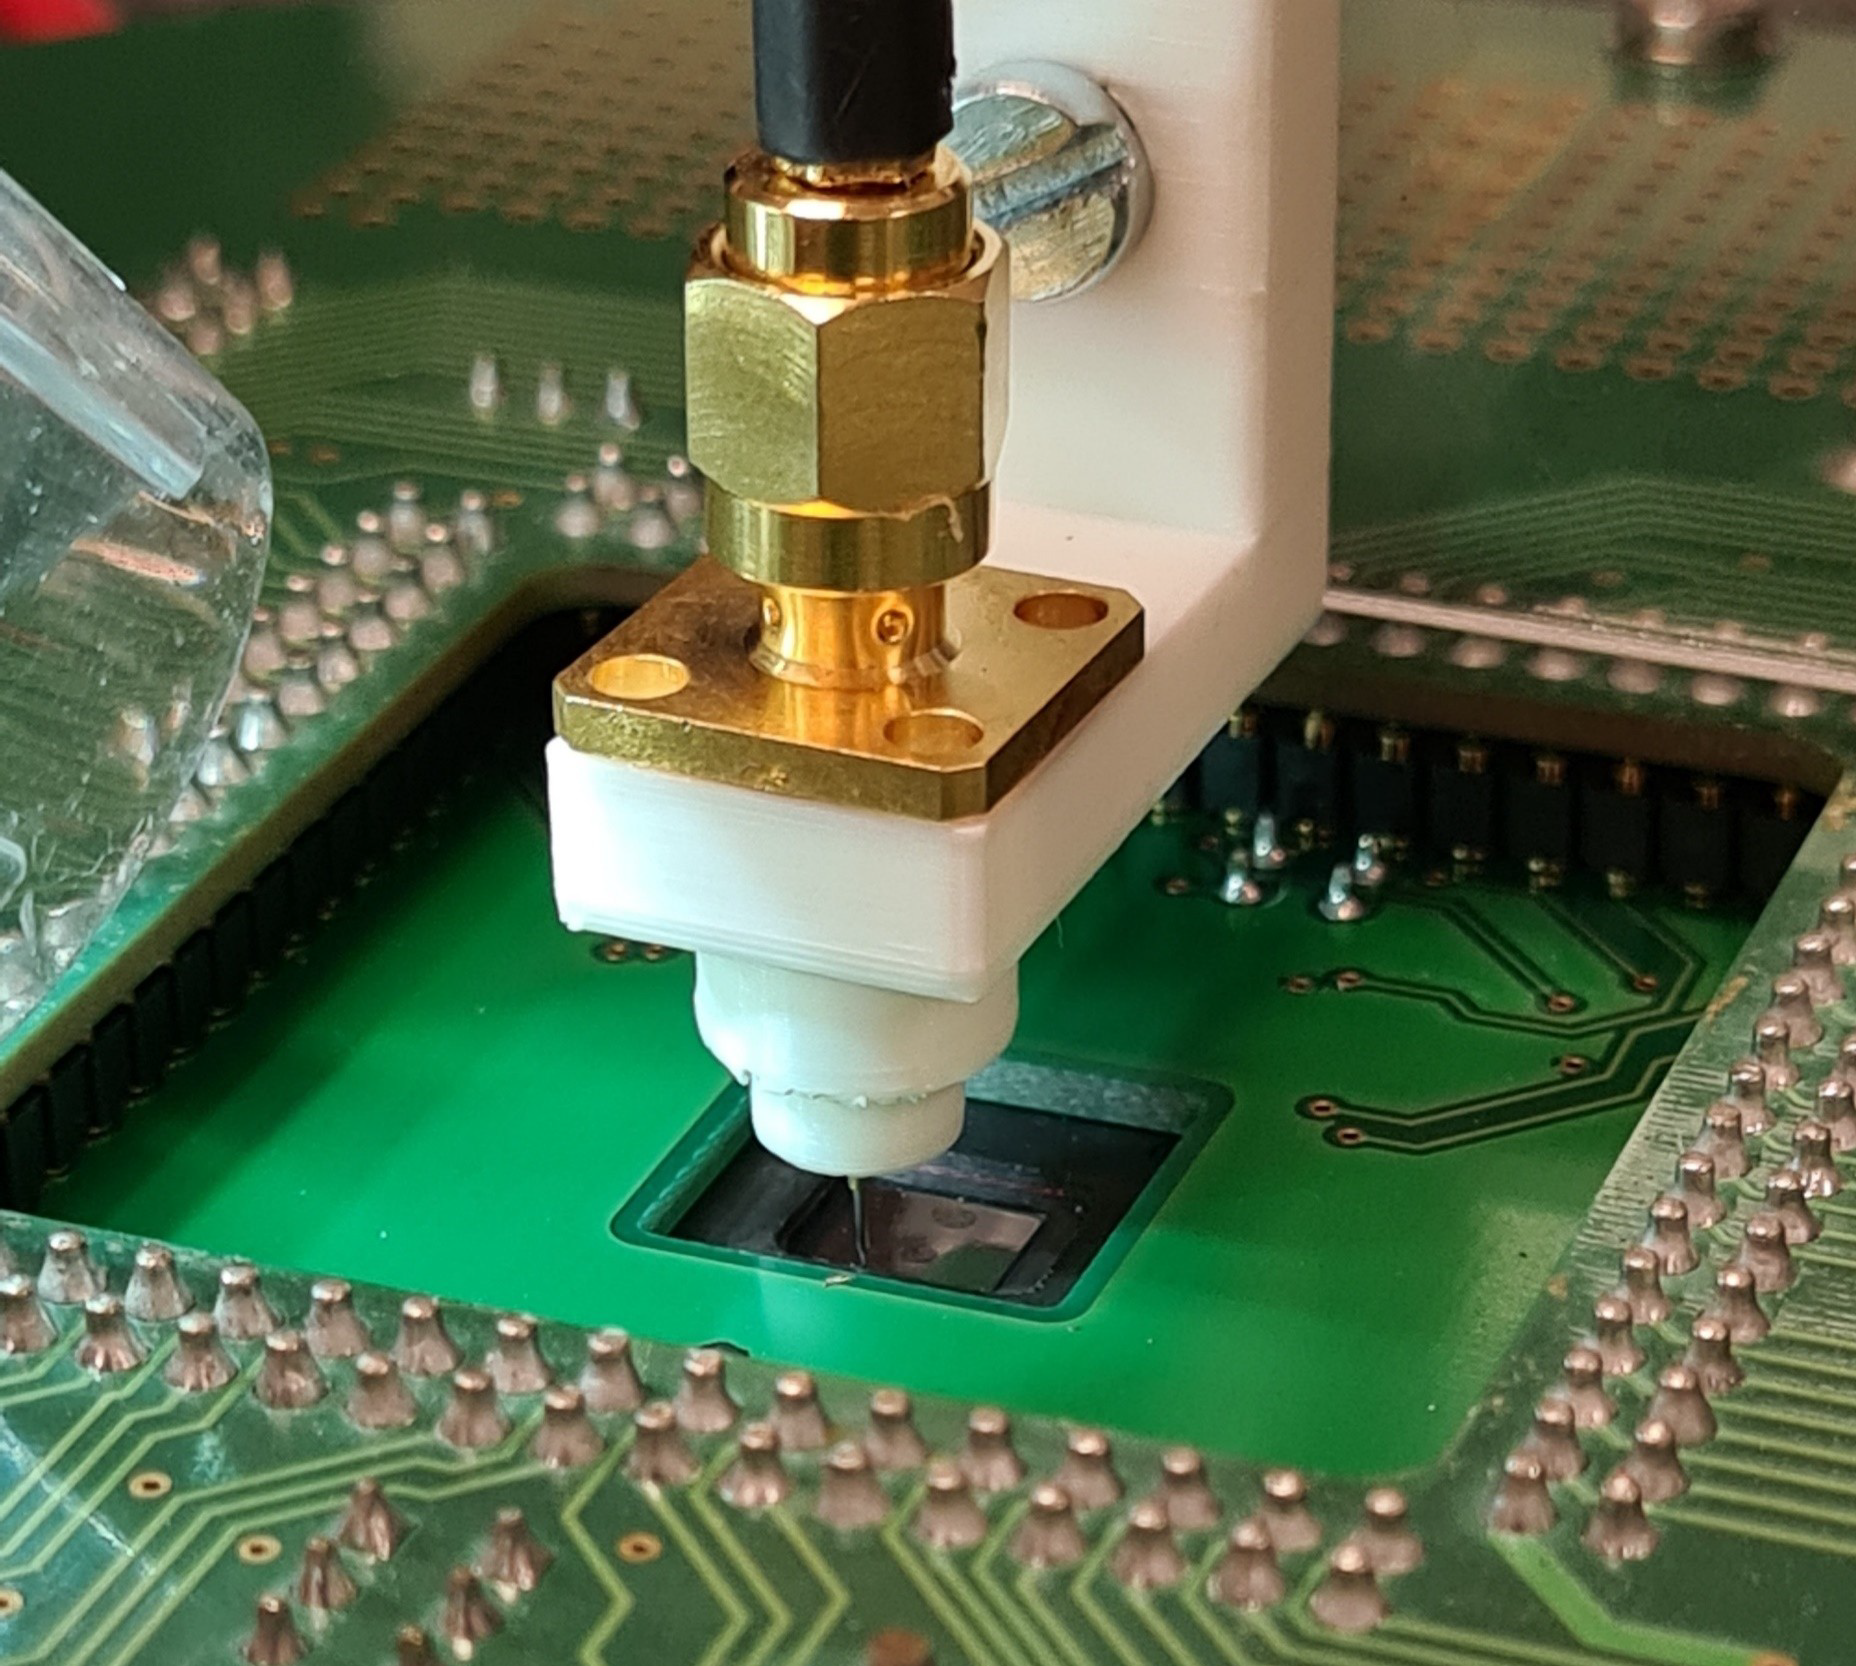
\includegraphics[width=16cm]{2_goodPractices/figures/sondeBBI_loin_raw.png}
%    \caption{BBI metallic probe in mechanical contact with IC target}
%    \label{fig:sondeBBI}
%\end{figure}
%
%\begin{figure}[H]
%    \centering
%    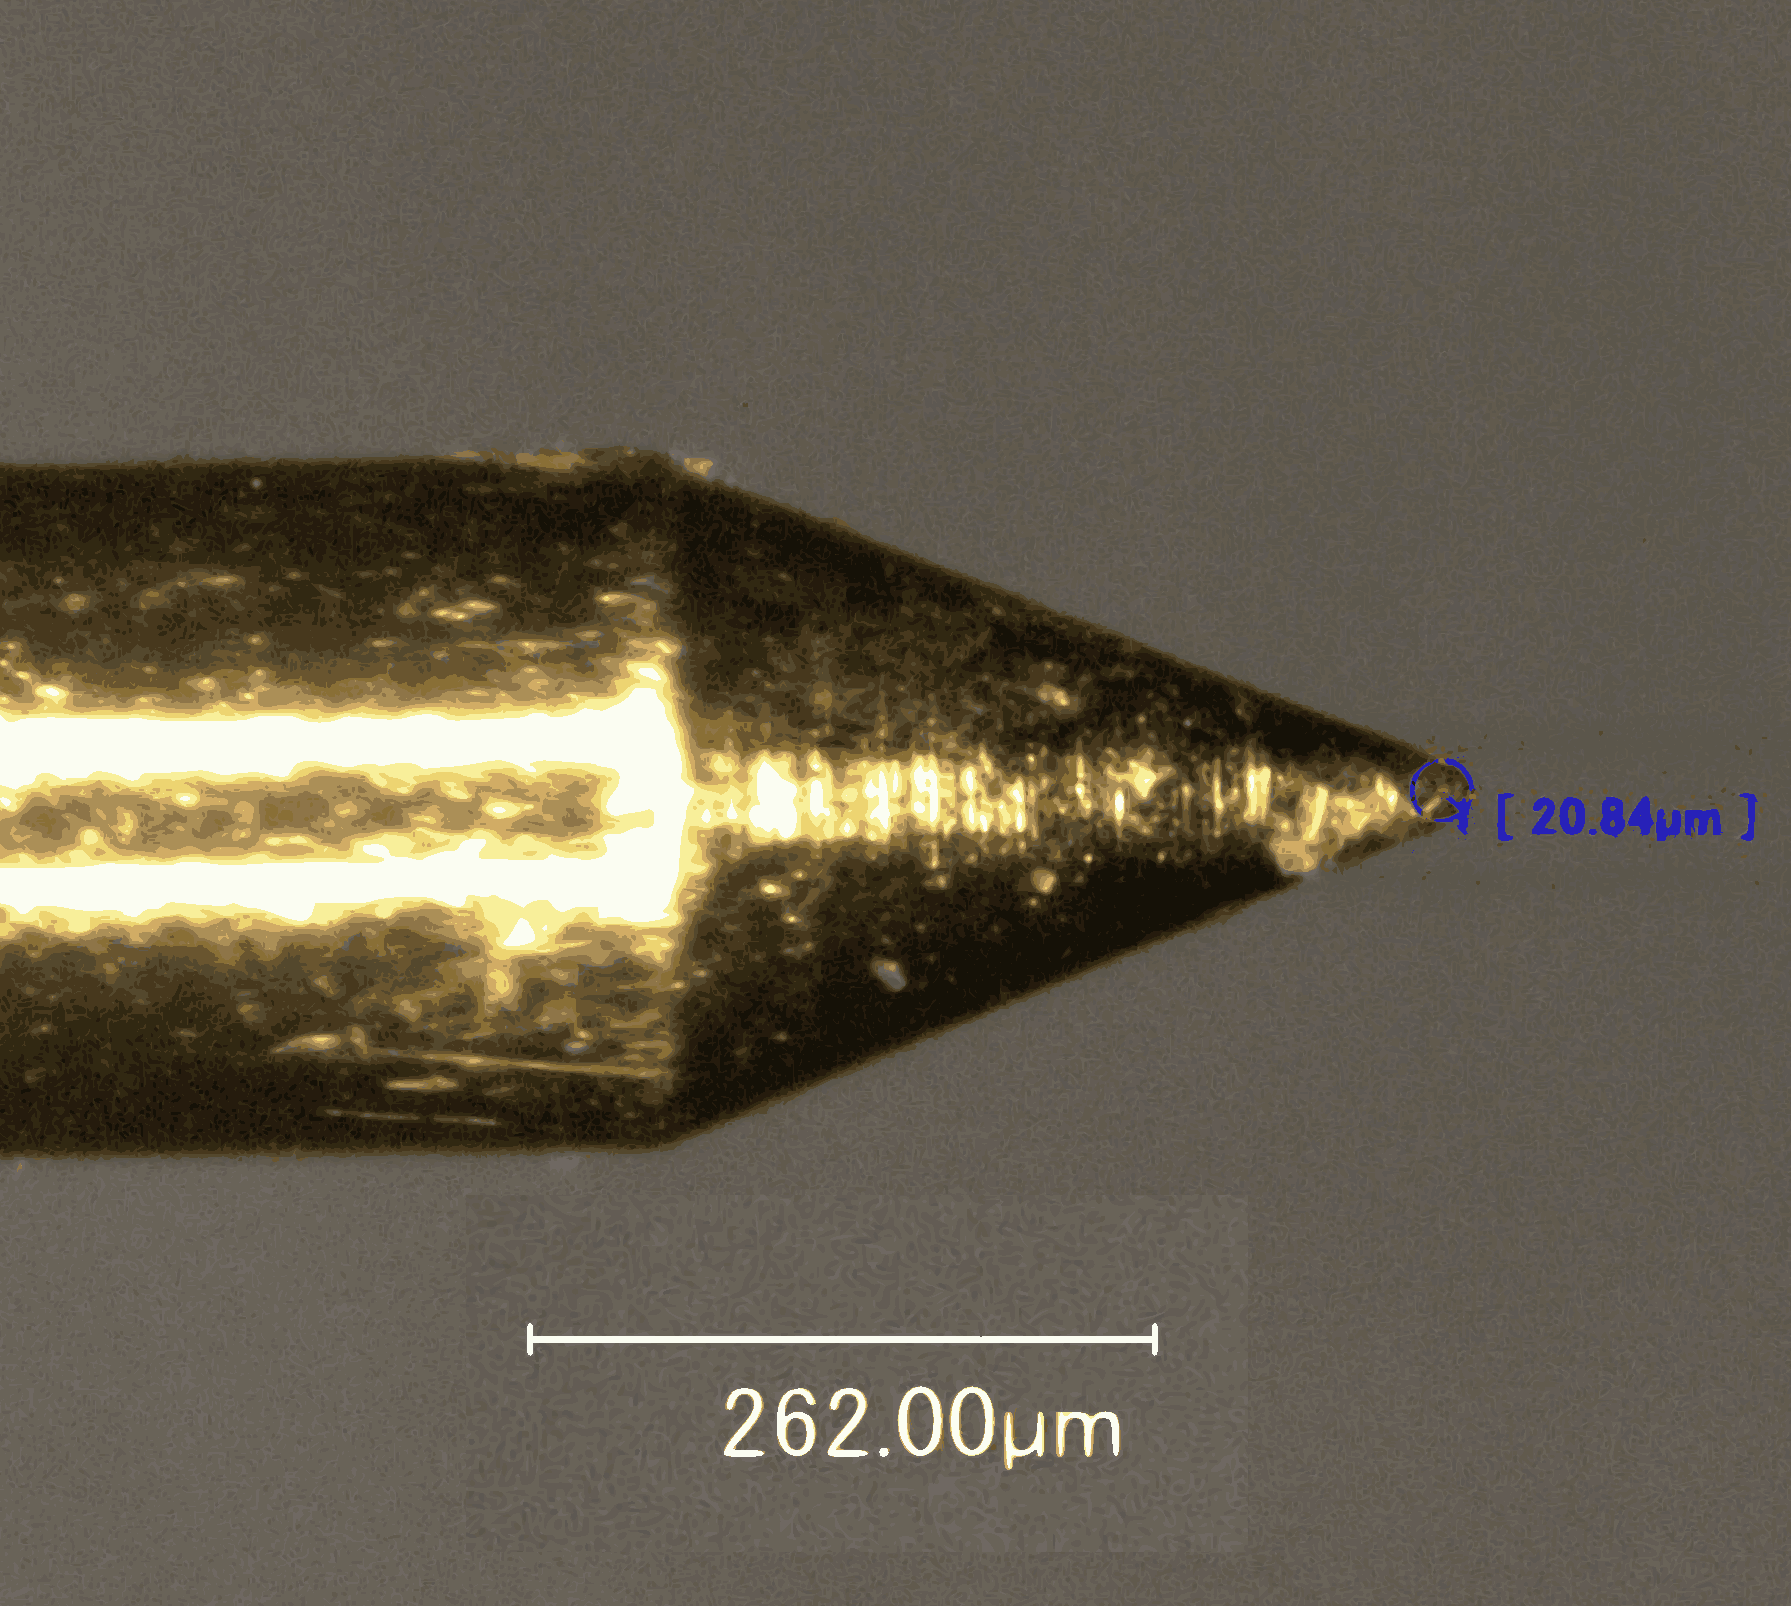
\includegraphics[width=16cm]{2_goodPractices/figures/pointeBBI.pdf}
%    \caption{BBI metallic probe measurement closer look}
%    \label{fig:pointeBBI}
%\end{figure}

\begin{figure}[ht!]
    \centering
    \begin{subfigure}[t]{7.0cm}
        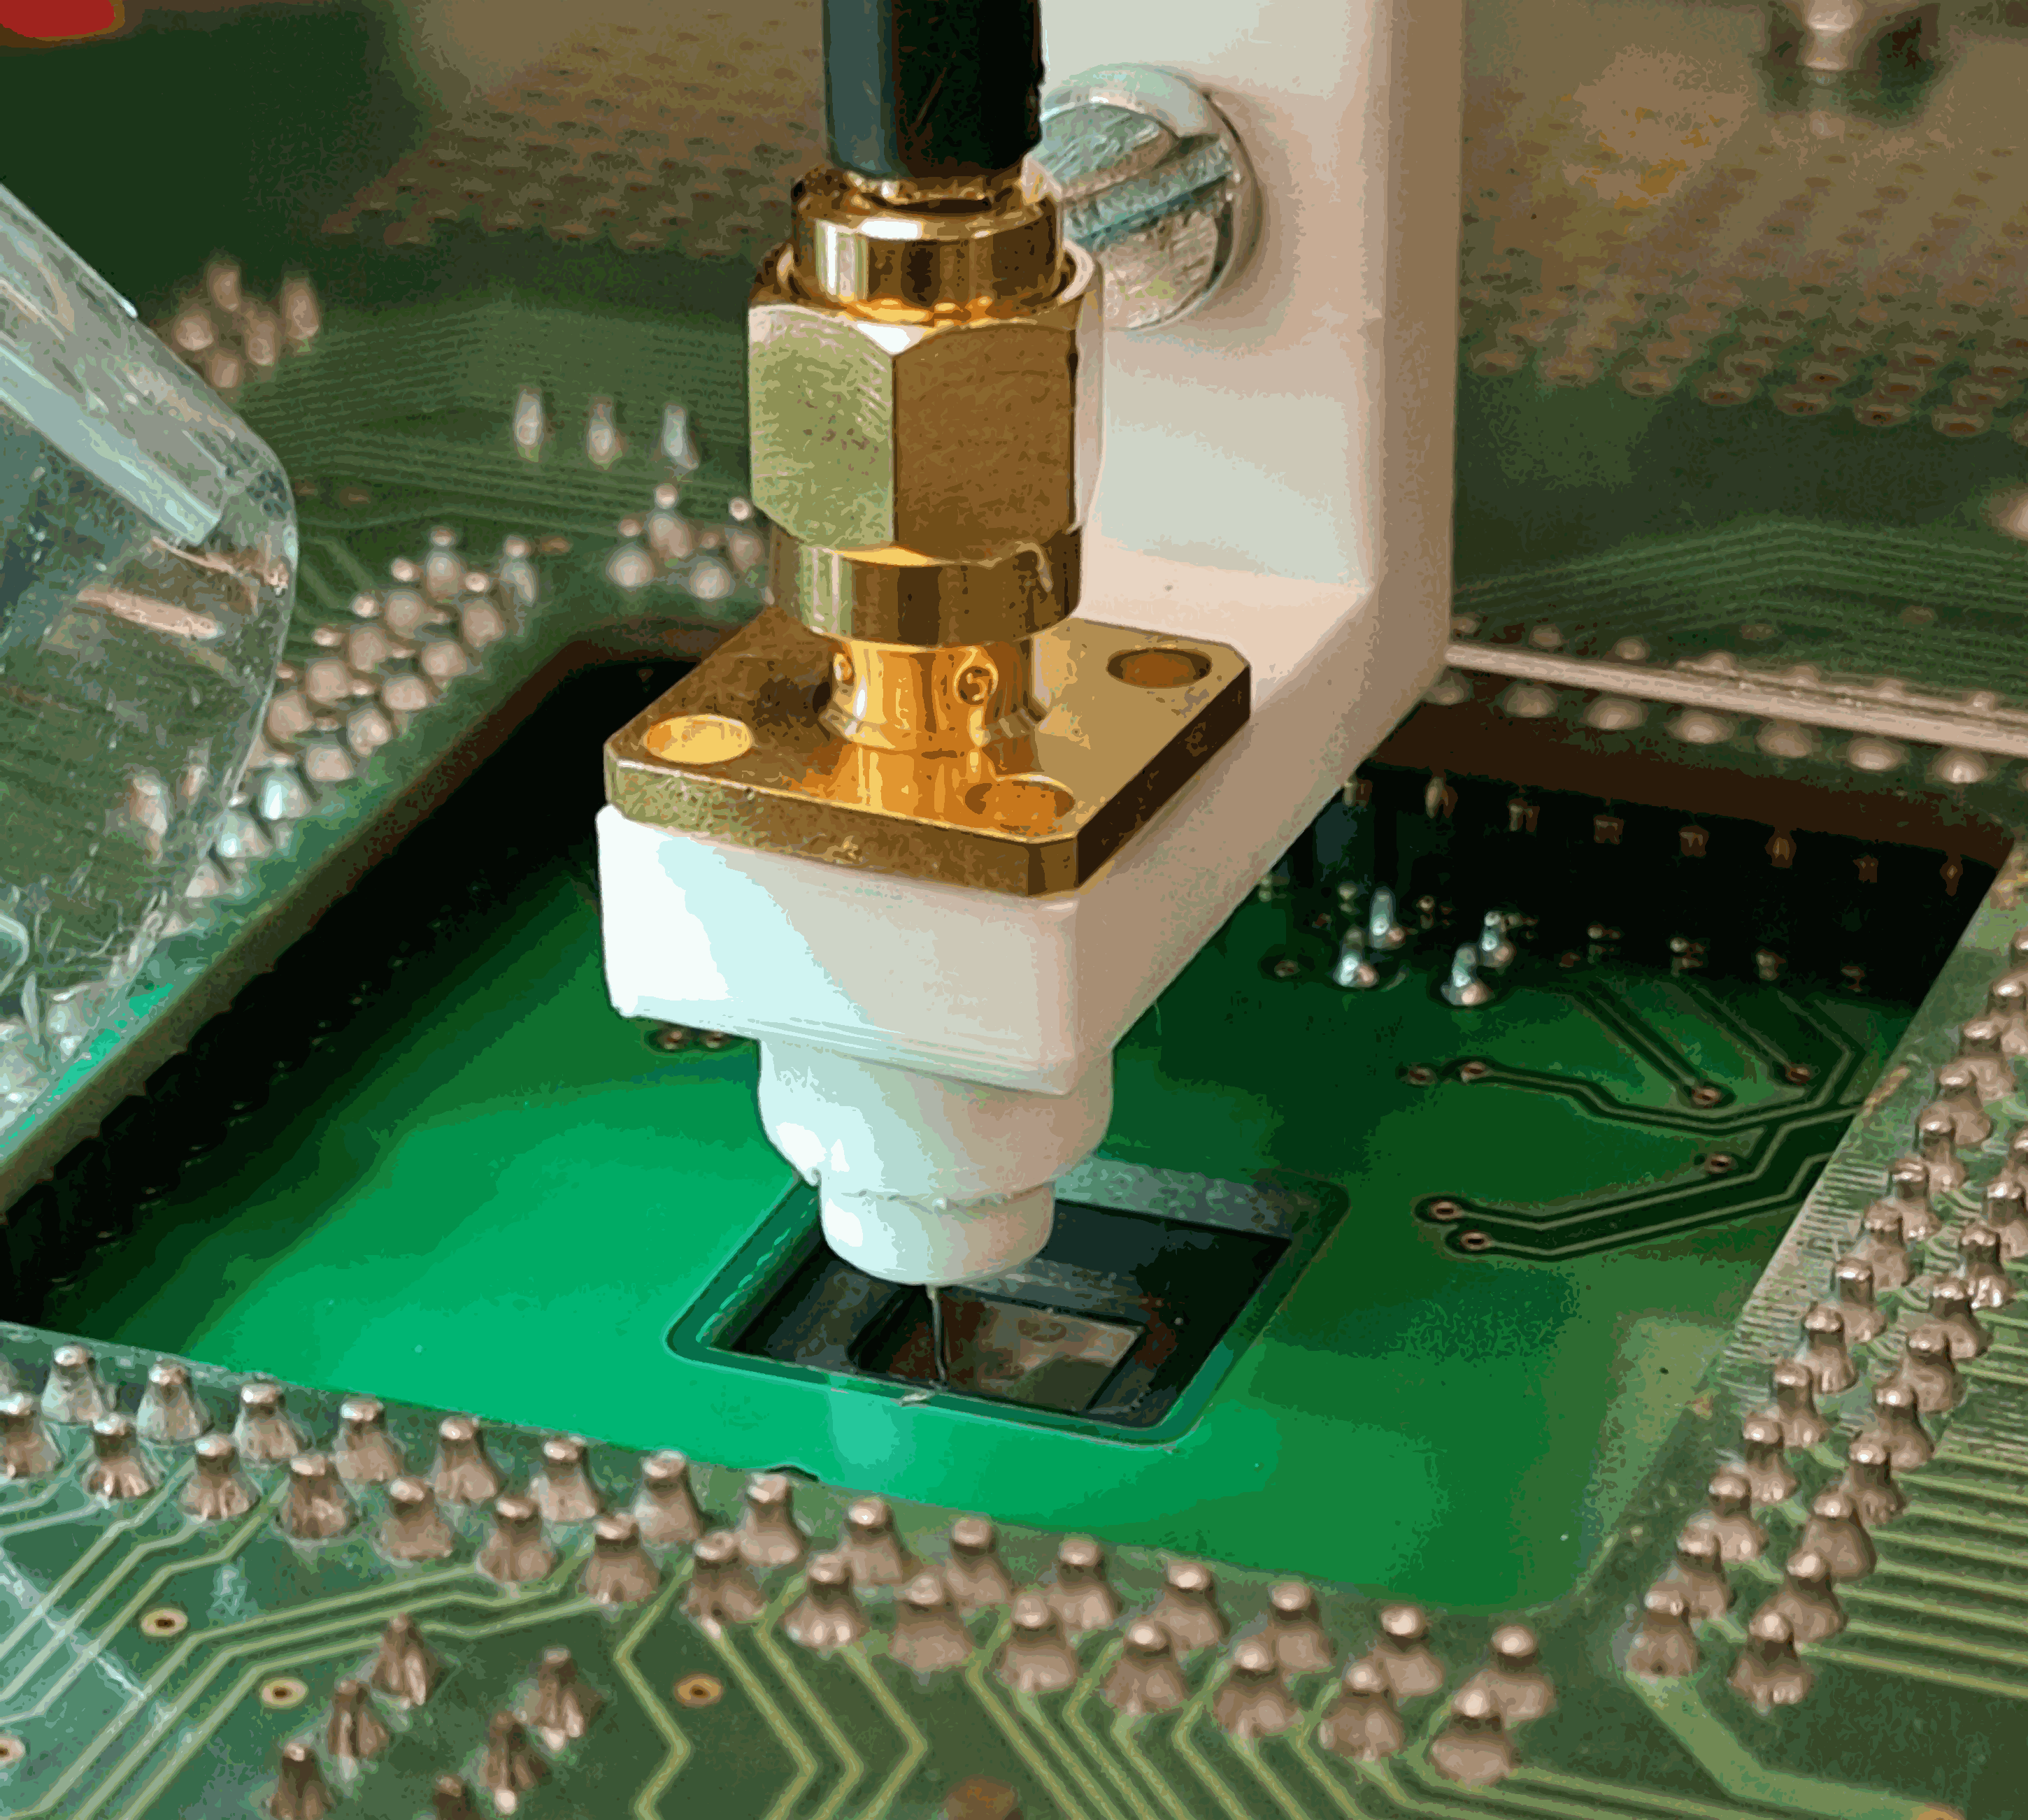
\includegraphics[height=6.8cm]{2_goodPractices/figures/sondeBBI.pdf}
        \caption{BBI metallic probe in mechanical contact with IC target}
        \label{subfig:sondeBBI}
    \end{subfigure}\hfill
    \begin{subfigure}[t]{7.0cm}
        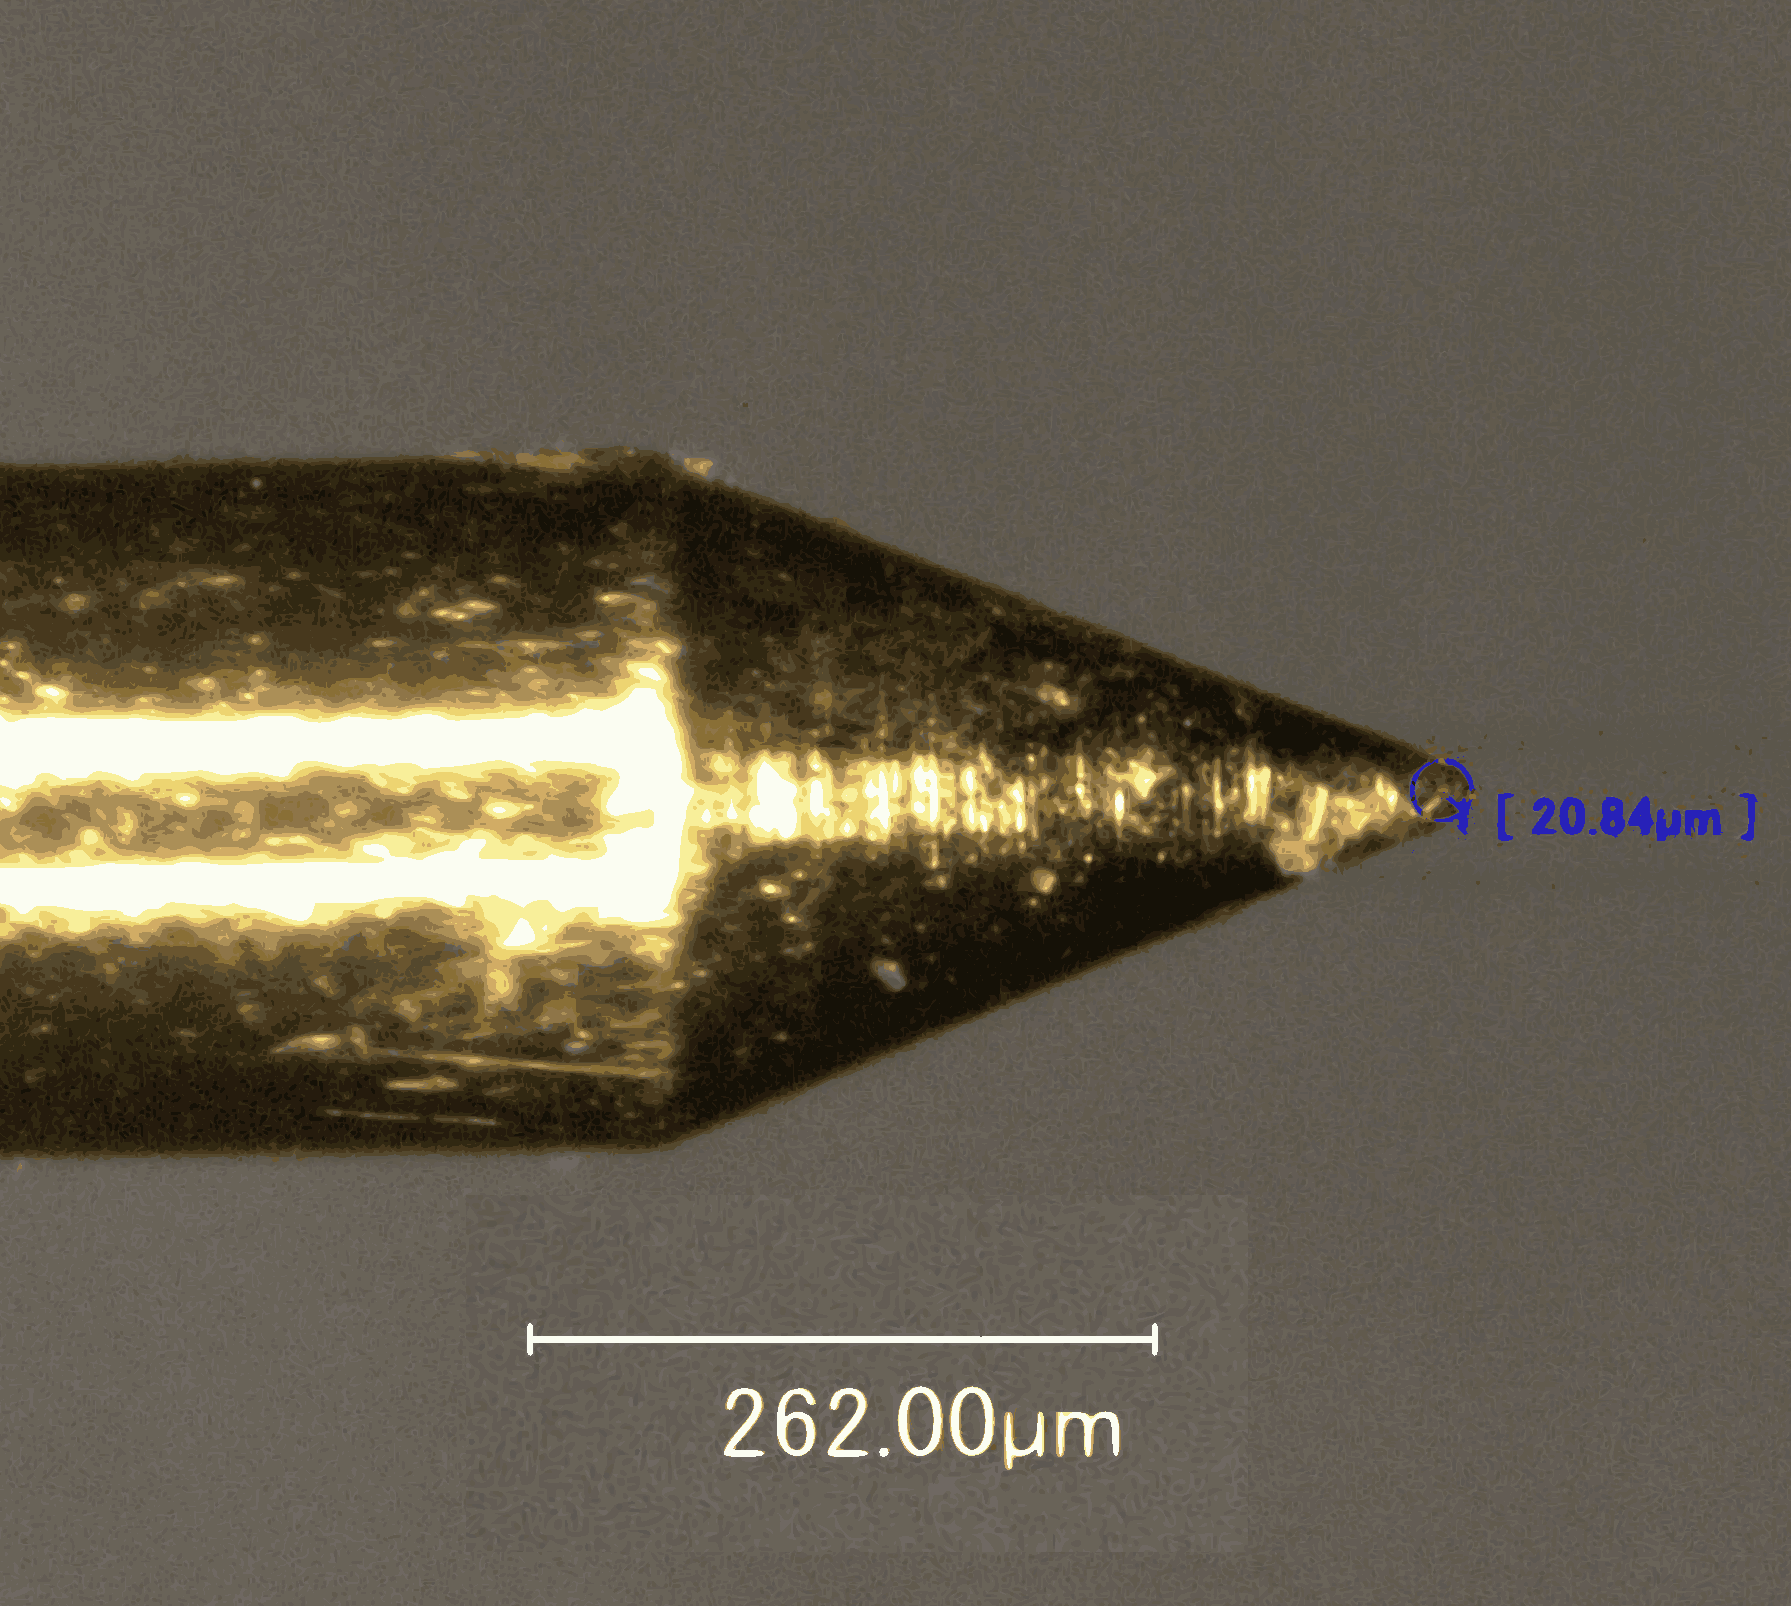
\includegraphics[height=6.8cm]{2_goodPractices/figures/pointeBBI.pdf}
        \caption{BBI metallic probe measurement closer look}
        \label{subfig:pointeBBI}
    \end{subfigure}
    \caption{Dual-well and triple-well inverter silicon sectional view.}
    \label{fig:sondePointeBBI}
\end{figure}

The main piece of equipment when working with BBI is the electrical probe.
It is commonly made with a metal tip, a connector of any sort and a mechanical support to hold everything together.
For the purpose of this work, a custom probe was designed around three simple parts, an SMA connector, in order to have a low-cost, small and standard interconnection, a spring-loaded metallic probe soldered onto the SMA connector, and a custom 3D printed support to hold the structure together.
Fig. \ref{fig:sondePointeBBI} shows detailed pictures of the designed BBI metallic probe, with a global view in operation on Fig.\ref{subfig:sondeBBI}, and a photograph under a microscope of the probe's tip-end on Fig. \ref{subfig:pointeBBI}, allowing to measure its actual size before the first usage.
The metallic probe used has a 0.635 mm diameter and is 16.35 mm long. The specified maximum nominal current of the probe is of 1.5 A, and the electrical contact resistance measures 70 m\textOmega.


\begin{figure}[H]
    \centering
    \includegraphics[width=\textwidth]{2_goodPractices/figures/picoemp-red.jpeg}
    \caption{ChipSHOUTER\textregistered-PicoEMP from NewAE Technology Inc.}
    \label{fig:newAeChipShouter}
\end{figure}
Another fundamental piece of equipment for the practice of BBI is the voltage pulse generator.
It is, generally, the most expensive hardware tool required.
However, nowadays, cheap solutions are easily available, like the NewAE Technology Inc. ChipSHOUTER\textregistered-PicoEMP for example, illustrated in Fig. \ref{fig:newAeChipShouter}.
In addition to being cheaper than most industrial solutions, its design sources are available online, making it a future-proof solution.
In contrast to more expensive solutions, it has inevitably some drawbacks:
\begin{itemize}
    \item The output transformer is low-power, around up to 200 mW
    \item Its recovery time is slow, from 1 to 4 seconds between pulses
    \item It can generate maximum voltage pulses of approximately 250 V
    \item There is no pre-calibration
    \item The pulse width control is not as reliable as other solutions
\end{itemize}
%Nonetheless, during this work, the generator used is the AVTECH AVRK-4-B, which a high speed, precise, voltage pulse generator.
%It allows generating positive or negative pulses up to 750 V of amplitude with a 4 ns rise or fall time, with pulse widths ranging from 6 ns to 20 ns.
%It allowed us to finely tune each setting in order to perform reproducible experiments.
%
%Another very important piece of equipment used for BBI is the probe.
%It simply consists in a metallic tip soldered to an SMA connector.
%However,

\section{Body Biasing Injection enhanced practice \DDC}
\label{chap2:goodPractices}
% !TeX root = ../0_Manuscript.tex

\section{Giraud's differential fault attack \ddc}
\label{chap:2_goodPractices;sect:dfaGiraud}
Now that we have seen the benefits of the proposed practice with a simple experiment, it is required, to further support these outcomes, to conduct in-depth experiments.
To that end, we propose to compare the conduct and outcome of a differential fault attack, specifically the mono-bit Giraud's DFA as defined in the third section of \cite{giraudDfa}.

% !TeX root = ../0_Manuscript.tex
%    trim={left lower right upper}
%\begin{figure}[H]
%    \centering
%%    \includegraphics[width=0.5\textwidth,
%%    trim={20cm 0cm 0cm 0cm},
%%    center]{2_goodPractices/figures/aesFastImpGnd.pdf}
%    \includegraphics[width=0.8\textwidth, center,
%    trim={14.9cm 0cm 0cm 0cm}, clip]{2_goodPractices/figures/aesFastImpGnd.pdf}
%    \caption{Fault susceptibility map analysis}
%    \label{fig:giraudFSM}
%\end{figure}

\begin{figure}[H]
    \centering
    \begin{subfigure}{0.49\textwidth}
        \includegraphics[width=\textwidth, center,
        trim={14.9cm 0cm 0cm 0cm}, clip]{2_goodPractices/figures/aesFastGndOnly.pdf}
        \caption{FAM: state-of-the-art}
        \label{fig:gndFSM}
    \end{subfigure}
    \begin{subfigure}{0.49\textwidth}
        \includegraphics[width=\textwidth, center,
        trim={14.9cm 0cm 0cm 0cm}, clip]{2_goodPractices/figures/aesFastImpGnd.pdf}
        \caption{FAM: enhanced}
        \label{fig:giraudFSM}
    \end{subfigure}
    \caption{Fault analysis mapping}
    \label{fig:fam}
\end{figure}


\textcolor{orange}{CARTOS À FAIRE...}
% !TeX root = ../0_Manuscript.tex

\chapter{Integrated circuits modeling \ddcip}
\label{chap:3icModeling}
\vspace{-3cm}
\minitoc
\newpage


\section{Summary \ddcu}
%This chapter presents the work carried out concerning the modeling and simulation of integrated circuits and platforms in a body biasing fault injection context.
%The presented work focused on elaborating electrical models allowing to evaluate with simulations the behaviors of ICs subjected to BBI.
%The chapter introduces the elaborated models and the algorithms used to create them, and then goes on to present various validation steps to check the meaningfulness of the models.

%This chapter introduces and develop the work carried out concerning the integrated circuit modeling in a \bbi context.
%It begins with an introduction of the various aspects on how IC are manufactured, including power delivery networks and silicon substrate types, depicting the main aspects of their structure.
%Afterward, it introduces electrical models allowing to simulate integrated circuits under \bbi.
%Then, it lingers on how to properly model the voltage pulse generator and the electrical probe, which are the main tools for performing \bbi.
%Eventually, it shows the study of how actual logic gates react to \bbi disturbances and the implications of such results.
%Parts of this work have been published both in \cite{mybbiCosade} and \cite{mybbiFdtc2022}.

This chapter is dedicated to introducing the work I carried out concerning the modeling and simulation of integrated circuits, subject to \bbi.
It begins with a discussion of the various aspects involving how ICs are designed and manufactured.
It includes a thorough description of their power delivery network and silicon substrate.
The main aspects of their structure, being inherited from the standard design flow provided by CAD vendors, are also described.
Afterward, it introduces electrical models allowing to simulate integrated circuits under \bbi.
Then, it lingers how to properly model the voltage pulse generator and the electrical probe, which are the main tools for performing \bbi.
Eventually, it shows the study of how actual logic gates react to \bbi disturbances and the implications of such results.
Parts of this work have been published both in \cite{mybbiCosade} and \cite{mybbiFdtc2022}.


\section{Introduction \DDC}
When evaluating and studying ICs under BBI, it is important to be able to fully predict and understand the underlying mechanisms at work in order to set up reproducible and reliable experiments, as well as being able to set up efficient countermeasures.
However, to model and simulate integrated circuit behavior subject to fault injection is not an easy task.
Specifically, simulating an entire IC at a transistor level under fault injection is unrealistic with current resources and technology.
It is especially true when considering time cost, as current digital ICs are composed of about a million of transistors for standard microcontrollers.
Furthermore, no software nor algorithm is currently dedicated to simulate the functional, electrical behavior of millions of transistors at the same time while some of them are disrupted by strong and transient disturbances.
In addition to that, to be able to set up a reliable model, one should have access to the detailed architecture of each considered IC, which is almost never the case, as most studied architectures are proprietary.
Therefore, it is required to find alternative workarounds in order to be able to study IC behavior and their various responses to fault injection techniques.

This has been first proposed in 2019 concerning Electromagnetic Fault Injection (EMFI) \cite{mathieuEMFIFirst}, and further extended in 2021 \cite{mathieuEMFI}.
Especially in the latest work \cite{mathieuEMFI}, the proposed solution consisted in establishing an equivalent non-logical model of the section of an IC.
Instead of modeling each logic gate with as many transistors as required, in addition to the power delivery network and the silicon substrate, it was chosen to represent a hundred of logic gates in an average way, solely with a few resistors and capacitors.
This results in a transistor-less model, achieved using manufacturing data for the studied IC.
The authors assumed that the first half of the transistors are conducting while the other half are blocking.
Then, two levels of power delivery network were added, simply modeled with electrical resistances.
Eventually, and because the modeled IC was manufactured using a dual-well substrate type, the silicon substrate and the P-N junction respectively are modeled by six resistors going in every direction in addition to a diode and its capacitance respectively.
This clever design allows to drastically reduce the computing work required to analyze and predict behaviors of ICs subject to EMFI.
Indeed, simulating the average behavior of a hundred of logic gates only with four resistors and four capacitors is immensely lighter than simulating the equivalent with BSIM (Berkeley Short-channel IGFET Model) transistors.
However, the main shortcoming being the lack of functionality with the produced ICs, it is therefore impossible to evaluate their functional or logical behavior.

Body biasing injection being less documented than EMFI, no distributed model has yet been proposed to simulate ICs under BBI.
In this context, our motivations were to set up and evaluate electrical models being able to reliably predict both in time and space IC behavior in order to understand how BBI induced disturbances propagate and create faults inside ICs.
The current work main goal being to model and simulate BBI similarly to EMFI, we decided to start from the model proposed in \cite{mathieuEMFI}, to improve and adapt it in order to be able to implement it in a BBI context.
%The main goal of the current work being to model and simulate reliably BBI, and as no model was proposed for BBI as it is more recent and less documented than EMFI, we decided, based on the models from \cite{mathieuEMFI}, to improve them in order to be able to use them in a BBI environment.

This chapter begins with a general presentation of the enhanced models, followed by a closer look at each model and its specific features.
Eventually, various model validation are studied in order to verify their soundness.


\section{Integrated circuits structure \ddcnew}
For the purpose of properly introducing the electrical models I developed for \bbi, it is required, in the first place, to linger on how integrated circuits are structured.
It involves analyzing the main structures composing an IC, such as:
\begin{itemize}
    \setlength\itemsep{-0.1em}
    \item Its power supply network, consisting in various metal levels stacked one on top of the others;
    \item The standard-cells: pre-characterized logic cells used as elementary building blocks;
    \item The various substrate types, such as \dwF and \twF that I considered in my work, not to cite them all.
\end{itemize}

    \subsection{Power supply rails \ddcnew}
    \begin{figure}[ht]
    \centering
    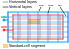
\includegraphics[width=0.45\textwidth]{3_modeling/figures/IC_POWER_PLANS.pdf}
    \caption{Coarse traditional IC power delivery diagram, showing a standard-cell segment sandwiched between power rails.}
    \label{fig:icPowerRail}
\end{figure}
    In most modern integrated circuits, power is brought to the transistors through various metal layers organized as meshes.
%    The resulting meshes bring the power to the transistors, aka the logic gates, aka the Standard-Cells.
    In digital ICs, there is typically two power delivery signals, commonly called VDD and GND, GND being the ground reference of the IC.
    There are one or more pads for each power signal, connecting to power rings, surrounding the IC silicon die, as shown in Fig. \ref{fig:icPowerRail}.
    Then, power straps are created to mesh the rings and distribute evenly the power to the transistors.
    After that, rails are drawn to connect the power to the standard-cell segments, and vias are placed between rails and straps to wire them together.

    \subsection{Standard-Cell rows \ddcnew}
    \begin{figure}[ht]
    \centering
    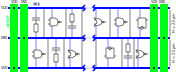
\includegraphics[width=0.55\textwidth]{3_modeling/figures/std_cell_segment_principle.pdf}
    \caption{Symbolic view of a Standard Cell Segment, surrounded by its local power delivery network.}
    \label{fig:istdCellRows}
\end{figure}
    As previously mentioned, Standard-Cells are the elementary building blocks used to design ICs.
    They are pre-defined logic cells, fulfilling a specific logic function.
    Standard-Cells can then be connected together to form a complete logic function.
    They are usually organized in rows, with a fixed height and variable width depending on the function.
    This allows simple power connection to each Standard-Cell.
    Fig. \ref{fig:istdCellRows} illustrates how Standard-Cells are connected to the power supply network in an IC design.
    At the top of the Standard-Cells is the VDD power input, and at the bottom the GND power input.
    Typically, without considering various technologies, between the power rails are trapped three main regions:
    \begin{itemize}
        \setlength\itemsep{-0.1em}
        \item A N-doped silicon area, called the N-well, where the PMOS transistors are lithographed;
        \item A metal area where the transistor gates are accessible;
        \item A P-doped silicon area, called the P-well, where the NMOS transistors are lithographed.
    \end{itemize}
    Therefore, NMOS transistors are located in the bottom half of the standard-cell, and the PMOS are located in the top half.

    \subsection{Various substrate types \ddcnew}
    \begin{figure}[htbp!]
    \centering
    %\scriptsize
    % \setstretch{0.9}
    \begin{subfigure}{7.8cm}
        % \def\svgwidth{9.0cm}
        \includegraphics[width=7.8cm]{3_modeling/figures/DUAL.pdf}
        \caption{Dual-Well}
        \label{subfig:dualIvx}
    \end{subfigure}
    \begin{subfigure}{7.8cm}
        % \def\svgwidth{9.0cm}
        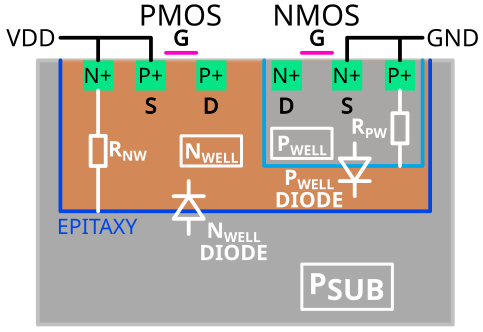
\includegraphics[width=7.8cm]{3_modeling/figures/TRIPLE.pdf}
        \caption{Triple-Well}
        \label{subfig:tripleIvx}
    \end{subfigure}
    \caption{Dual-well and triple-well inverter silicon sectional view.}
    \label{fig:dualTripleIvx}
\end{figure}
    Because there are various ways to lithograph transistors for a given technology, I decided to linger and analyze the differences of two substrate types commonly found in bulk technologies:
    \begin{itemize}
        \setlength\itemsep{-0.1em}
        \item \dwF substrates, where NMOS transistors are lithographed directly into the P-doped silicon substrate;
        \item \twF substrates, where the NMOS transistors are lithographed into a buried P-well inside the N-well where the PMOS are lithographed.
    \end{itemize}
    For the purpose of illustrating the structural differences between those substrate types, I am going to use the schematics displayed in Fig. \ref{fig:dualTripleIvx} as a guide, illustrating the cross-sectional view of a logic inverter created in both a \dwF and a \twF substrate.

        \subsubsection{\dwF substrates \ddcnew}
        To begin with, let us focus on \dwF substrates.
        A schematic sectional view of a CMOS inverter manufactured in a \dwF substrate is shown in Fig. \ref{subfig:dualIvx}
        Among moderately old ICs, it was common to find \dwF substrates.
        In these substrates, NMOS transistors are lithographed directly into the P-doped silicon substrate, as we can see in Fig. \ref{subfig:dualIvx}.
        In addition to this, a N-doped silicon area is created inside the P-substrate, called the N-well, to lithograph the PMOS transistors.
        This results in a silicon junction, electrically represented by the N-well diode on the schematic, and called the epitaxy, highlighted in saturated blue.
        Because doped silicon does have a non-zero resistivity, electrical resistances are represented to demonstrate this:
        \begin{itemize}
            \setlength\itemsep{-0.1em}
            \item $RC_{VDD}$ represents the access resistance measured between the epitaxy and the PMOS transistor through the N-well;
            \item $RC_{GND}$ is the access resistance measured between the epitaxy and the NMOS transistor through the P-substrate.
        \end{itemize}

        \subsubsection{\twF substrates \ddcnew}
        \textcolor{orange}{TW helps to reduce crosstalk noise.}
        On the other hand, \twF substrates are also commonly used, often in combination with \dwF on the same die, to provide an electrical isolation between NMOS and PMOS transistors.
        It is achieved by creating inside the N-well, another doped silicon area, inversely doped, called the P-well.
        Inside the latter are then lithographed the NMOS transistors, while the PMOS transistors are still lithographed inside the N-well.

\section{Standard-Cell Segment (SCS) and their models \ddcnew}
Thanks to what I have introduced in the previous section, that is, the Standard-Cell arrangement used to create IC architectures, alongside the two identified substrate types of interest: \dwF and \twF, it is now possible to elaborate an electrical model for such integrated circuits.
Because I am differentiating \dwF and \twF substrates, I am introducing two separate models, even though they show some similarities.

The models I developed are an improvement over the electrical models proposed by M. Dumont for \emfi \cite{mathieuEMFI}.
Similar to \cite{mathieuEMFI} and to VLSI design, I am using the Standard-Cells as a basic building block.
However, in my model is not represented the logic function of a Standard-Cell, rather its electrical behavior.
More specifically, the elementary building block of the proposed electrical model represents the average electrical behavior of several Standard-Cells, called Standard-Cell Segment (\scs).

\begin{figure}[ht]
    \centering
    \includegraphics[width=0.65\textwidth]{3_modeling/figures/substrateSubdivision_6.pdf}
    \caption{Substrate subdivision improvement over M. Dumont model for \emfi \cite{mathieuEMFI}. The backside is the accessible substrate, and the epitaxy is the highest substrate level, a.k.a. the silicon junction between the P-substrate and the N-well.}
    \label{fig:surfaceSubDivid}
\end{figure}
Because I based my work on M. Dumont model \cite{mathieuEMFI}, there is a common base to which I have made modifications.
The major one consists in improving the model geometric accuracy in the case of \bbi studies.
In M. Dumont model, the silicon P-substrate is represented solely thanks to a network of 6 resistors, 30 µm wide, 5 µm long, and $t_{Sub}$ deep, $t_{Sub}$ being the entire modeled IC substrate thickness.
However, when performing \bbi, the substrate is the main physical environment where the electric charges travel.
Therefore, as I describe in more details further, it is required to improve the spatial resolution of the model concerning the substrate, as shown in Fig. \ref{fig:surfaceSubDivid}.
This is done by splitting the substrate electric model in several 6-resistors elementary networks interconnected with each other.
It allows representing the same substrate with more resistors, thus enabling more precise analysis of the substrate charges distribution during \bbi.

\begin{figure}[ht]
    \centering
    %\scriptsize
    % \setstretch{0.9}
    \begin{subfigure}{0.45\textwidth}
        % \def\svgwidth{9.0cm}
        \includegraphics[width=\textwidth]{3_modeling/figures/dualWell_no_5e.pdf}
        \caption{Dual-Well}
        \label{subfig:dualScs}
    \end{subfigure}
    \hfill
    \begin{subfigure}{0.45\textwidth}
        % \def\svgwidth{9.0cm}
        \includegraphics[width=\textwidth]{3_modeling/figures/tripleWell_no_5e.pdf}
        \caption{Triple-Well}
        \label{subfig:tripleScs}
    \end{subfigure}
    \caption{Three-dimensional Dual-Well and Triple-Well IC comprehensive standard-cell electrical schematic.}
    \label{fig:dualTripleScs}
\end{figure}
%\begin{figure}[ht]
%    \centering
%    
\includegraphics[width=0.50\textwidth]{3_modeling/figures/logicGatesModelMathieu.pdf}
%    \caption{Electrical equivalent model of two inverters interconnected with each other.}
%    \label{fig_equivLogicGateStdCell}
%\end{figure}

\begin{figure}[ht]
    \centering
    \begin{subfigure}{0.52\textwidth}
        
\includegraphics[width=\textwidth]{3_modeling/figures/logicGatesModelMathieu.pdf}
        \caption{Electrical equivalent model of two inverters interconnected with each other, with the first one outputting a logical ONE value.}
        \label{sfig_equivCMOS}
    \end{subfigure}
    \hfill
    \begin{subfigure}{0.44\textwidth}
        
\includegraphics[width=\textwidth]{3_modeling/figures/stdCellLayoutSimple.pdf}
        \caption{Simplified top view of a Standard-Cell with two power rail metal levels. In blue are the logic interconnections inside the Standard-Cell.}
        \label{sfig_simpleSCS}
    \end{subfigure}
    \caption{Equivalent logic gates models used in the SCS model (\ref{sfig_equivCMOS}), and a simplified top view of a Standard-Cell with its size (\ref{sfig_simpleSCS}).}
    \label{fig_equivLogicGateStdCell}
\end{figure}
Fig. \ref{fig:dualTripleScs} shows the complete 3-dimensional schematics of the developed models for my thesis.
An analog simplified schematic representing the top view of a Standard-Cell is shown in Fig. \ref{sfig_simpleSCS} for understanding and clarity purposes. It describes the two levels of metal considered in my modeling (in orange and red), alongside the internal Standard-Cell interconnections in blue, with its size annotated.

The next subsections are dedicated to describing these models both for \dwF and \twF substrates.
Each SCS is 30 µm wide, 5 µm long and $t_{Sub}$ deep, the thickness of the power delivery network and the logic gates being ignored, as the substrate thickness is often big in front of the latter.
In my models, an SCS represents about a hundred of logic gates, where half of their transistors are conducting.

    \subsection{The case of \dwF substrates \ddcnew}
    Fig. \ref{subfig:dualScs} shows the electrical model of an SCS for \dwF substrates.
    Each SCS is delimited by the P-substrate at its bottom (\ovalbox{1}) and by the power rails at its top (\ovalbox{5}, \ovalbox{5'}).
    The dotted wires at the bottom of the substrate indicates that each substrate layer can be repeated as required to form the correct $t_{Sub}$ thickness.
    \dwF \scs are composed of six main regions, each one describing a part of an IC core sampling:
    \begin{itemize}
        \setlength\itemsep{-0.1em}
        \item Region \ovalbox{1} is the substrate resistive network, composed of several resistors, and being an isotropic environment;
        \item Region \ovalbox{2} is the P-substrate/N-well junction, modeled by a diode (DNW-PS) and its capacitance (CNW-PS), and is called the epitaxy, represented thanks to the blue net on the schematic. In addition to this, there is an access resistance from the epitaxy to the top of the N-well (VDD), representing the non-zero electrical resistance of N-doped silicon;
        \item Region \ovalbox{3} is the access resistance from the epitaxy up to the GND power rail, representing the non-zero electrical resistance of the P-doped substrate;
        \item Region \ovalbox{4P} is the model of the PMOS transistors, half of them being conducting. It consists in an access resistance RP from the VDD power-rail to the PMOS, and two capacitances, CGP being the load formed by the PMOS input capacitances, CGN the load formed by the NMOS input capacitances. Fig. \ref{sfig_equivCMOS} shows the model principle;
        \item Region \ovalbox{4N} is similar to \ovalbox{4P}: it is the model of the NMOS transistors, half of them being conducting. It consists in an access resistance RN from the GND power-rail to the NMOS, and two capacitances, CGP being the load formed by the PMOS input capacitances, CGN the load formed by the NMOS input capacitances. Fig. \ref{sfig_equivCMOS} shows the model principle;
        \item Region \ovalbox{5} and \ovalbox{5'} are the power network interconnections, represented on two metal levels, the colored ones being the first metal levels, the gray being the top metal level.
        \item Eventually, region \ovalbox{6} is simply the decoupling existing between both GND and VDD power rails.
    \end{itemize}

    \subsection{The case of \twF substrates \ddcnew}
    Fig. \ref{subfig:tripleScs} illustrates the \scs model for \twF substrates.
    The \scs are delimited, as before, by the P-substrate at their bottom and the power delivery network at their top.
    As for the \dwF model, the bottom dotted wires indicate that each substrate layer is repeated as needed to create the correct thickness required.
    The main difference between \dwF and \twF \scs models lies in the region \ovalbox{3}.
    First, let me describe every region:
    \begin{itemize}
        \setlength\itemsep{-0.1em}
        \item As for the previous model, region \ovalbox{1} is the silicon P-doped substrate;
        \item Region \ovalbox{2} is the N-well, created inside the P-substrate, with the junction (epitaxy) represented by a blue wire. It is composed of the diode DNW-PS, and its capacitance CNW-PS, alongside the N-well access resistance RNW from the epitaxy up to the VDD network;
        \item Region \ovalbox{3} is where the \twF model drastically differ from the \dwF one. As I have explained before, in \twF substrates, the NMOS transistors are lithographed inside an isolated P-doped region called the P-well. Therefore, region \ovalbox{3} describes the P-well, with an additional silicon junction modeled with the diode DNW-PW connected backward compared to DNW-PS, its capacitance CNW-PW, and the P-well access resistance RPW to GND;
        \item The three other regions are identical to the previous \dwF model.
    \end{itemize}

    \subsection{Writing the elementary models \ddcnew}
    \begin{figure}[H]
    \centering
    \includegraphics[width=0.5\textwidth]{3_modeling/figures/algoFigure5.png}
    \caption{Elementary substrate 3D netlist}
    \label{fig:algo}
\end{figure}
    After having abstractly created the models, I decided to write them using SPICE (Simulation Program with Integrated Circuit Emphasis) language.
    In addition to writing them, I calculated, thanks to the technology values of our IC targets, to calculate the substrate resistor values.
    Considering the substrate resistivity being $\rho = 0.01 \; \Omega \cdot m$, and the elementary block size being $W = \; \mu m$; $L = 5 \; \mu m$; $D = 10 \; \mu m$, it is trivial to calculate each resistance value $R_i$ thanks to the following equation:
    \begin{equation}
        \label{eqn_resistivity}
        R_i = \frac{\rho \cdot l}{S}
    \end{equation}
    Knowing that $L = W \equiv LW$ and that $D = LW$, we can first write that the vertical resistances will be four times the horizontal ones.
    Therefore, calculating one value of them gives the six values.
    Let us calculate the vertical resistances, which I will call $RH$:
    \begin{equation}
        RH = \frac{\rho \cdot \frac{D}{2}}{L \cdot W} = 2000 \; \Omega
    \end{equation}
    Therefore, the horizontal resistances are equal to $RL = 500 \; \Omega$.
    These calculations can be adapted as needed depending on the technology used.
    In addition to that, a substrate with a given thickness $t_{Sub}$ can be represented with virtually any number of layers.
    For example, one can reduce the number of layer by ten by adjusting the resistor values.
    It has the advantage to provide a lighter simulation, which will be faster to perform, at the cost of less accuracy.

    Previously, I have stated that an \scs is 30 µm wide.
    However, the elementary block I described is 5 µm wide.
    To achieve a 30 µm wide \scs, it is simply required to connect six of these blocks together to form a $W = 30 \; \mu m \cdot L = 5 \; \mu m \cdot D = 10 \; \mu m$ substrate, as it can be seen in Fig. \ref{fig:dualTripleScs} models.
    \begin{figure}[ht]
    \begin{small}
        \begin{Verbatim}[frame=single]
.subckt elementary_blocx6 D1 D2 D3 D4 D5 D6
+F1 F2 F3 F4 F5 F6 L R RE1 RE2 RE3 RE4 RE5 RE6
+U1 U2 U3 U4 U5 U6 VSUBCintC
XX1 D1 F1 L VSUBCintL2 RE1 U1 elementary_bloc
XX2 D2 F2 VSUBCintL2 VSUBCintL1 RE2 U2 elementary_bloc
XX3 D3 F3 VSUBCintL1 VSUBCintC RE3 U3 elementary_bloc
XX4 D4 F4 VSUBCintC VSUBCintR1 RE4 U4 elementary_bloc
XX5 D5 F5 VSUBCintR1 VSUBCintR2 RE5 U5 elementary_bloc
XX6 D6 F6 VSUBCintR2 R RE6 U6 elementary_bloc
.ends elementary_blocx6
        \end{Verbatim}
    \end{small}
    \caption{SCS substrate layer SPICE netlist}
    \label{fig_elemBlocX6}
\end{figure}
    The resulting netlist is shown in Fig. \ref{fig_elemBlocX6}, and naturally instantiate six times the previous netlist shown in Fig. \ref{sfig_spiceNetSub}.

\section{Integrated circuit modeling: interconnecting Standard-Cell Segments together \ddcnew}
Because the \scs I previously introduced only describe a portion of an integrated circuit, in order to model a complete one, it is required to instantiate several \scs and to connect them with each other in a mesh grid.
\begin{figure}[ht]
    \centering
    \includegraphics[width=0.5\textwidth]{3_modeling/figures/resultingSimulated_ic.png}
    \caption{Three-dimensional Standard-Cell Segments interconnection example.}
    \label{fig:surfaceSplitScs}
\end{figure}
Fig. \ref{fig:surfaceSplitScs} is a coarse illustration of what is done.
\scs are written, as the elementary substrate building blocks, in SPICE.
The \scs elementary models were automatically generated instead of being written manually, to avoid errors and enabling fast modifications to the models when required.
In addition to this, I decided to create an algorithm to connect as much \scs as needed to create a resulting IC.
By doing so, the interconnection process is once again automated and free from human errors.
A simple description of the algorithm is depicted in Alg. \ref{alg:icGen}
Because I have designed two separate models, one for \dwF and another for \twF substrate types, in addition to the various dynamic parameters which are useful when modeling an IC, the algorithm offers a certain degree of flexibility.
The actual program was written and implemented using Python, implementing procedural generation of integrated circuits according to the input parameters.
Next is the list of user-modifiable input parameters of the algorithm:
\begin{itemize}
    \setlength\itemsep{-0.1em}
    \item The resulting IC size;
    \item The \bbi probe location;
    \item The IC global substrate thickness;
    \item The substrate sub-model thickness;
    \item The substrate type: \dwF, \twF, or a mix of both, allowing to replicate actual IC architectures;
    \item The voltage pulse amplitude, width, and rise and fall times;
    \item Various SPICE simulation settings.
\end{itemize}
Eventually, the program incorporates a visual inspection tool in order to provide a quick verification of the generated IC structure to the end-user.

%As each \scs has external connections

%%%%%%%%%%%%%%%%%%%%%%%%%%%%%%%%%%%%%%%%%%%%%%%%%%%%%%%%%%%%%%%%%%%%%%%%%%%%%%%%%%%%%%%%%%%
%%%%%%%%%%%%%%%%%%%%%%%%%%%%%%%%%%%%%%%%%%%%%%%%%%%%%%%%%%%%%%%%%%%%%%%%%%%%%%%%%%%%%%%%%%%
%%%%%%%%%%%%%%%%%%%%%%%%%%%%%%%%%%%%%%%%%%%%%%%%%%%%%%%%%%%%%%%%%%%%%%%%%%%%%%%%%%%%%%%%%%%
%%%%%%%%%%%%%%%%%%%%%%%%%%%%%%%%%%%%%%%%%%%%%%%%%%%%%%%%%%%%%%%%%%%%%%%%%%%%%%%%%%%%%%%%%%%
%%%%%%%%%%%%%%%%%%%%%%%%%%%%%%%%%%%%%%%%%%%%%%%%%%%%%%%%%%%%%%%%%%%%%%%%%%%%%%%%%%%%%%%%%%%
%%%%%%%%%%%%%%%%%%%%%%%%%%%%%%%%%%%%%%%%%%%%%%%%%%%%%%%%%%%%%%%%%%%%%%%%%%%%%%%%%%%%%%%%%%%
%%%%%%%%%%%%%%%%%%%%%%%%%%%%%%%%%%%%%%%%%%%%%%%%%%%%%%%%%%%%%%%%%%%%%%%%%%%%%%%%%%%%%%%%%%%
%%%%%%%%%%%%%%%%%%%%%%%%%%%%%%%%%%%%%%%%%%%%%%%%%%%%%%%%%%%%%%%%%%%%%%%%%%%%%%%%%%%%%%%%%%%

%\section{Electrical models \ddcold}
%\label{sect:elecModels}
%%\begin{figure}[htbp!]
    \centering
    %\scriptsize
    % \setstretch{0.9}
    \begin{subfigure}{7.8cm}
        % \def\svgwidth{9.0cm}
        \includegraphics[width=7.8cm]{3_modeling/figures/DUAL.pdf}
        \caption{Dual-Well}
        \label{subfig:dualIvx}
    \end{subfigure}
    \begin{subfigure}{7.8cm}
        % \def\svgwidth{9.0cm}
        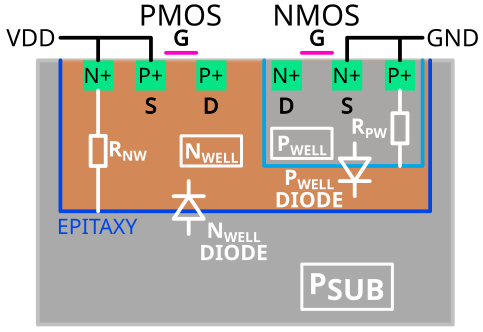
\includegraphics[width=7.8cm]{3_modeling/figures/TRIPLE.pdf}
        \caption{Triple-Well}
        \label{subfig:tripleIvx}
    \end{subfigure}
    \caption{Dual-well and triple-well inverter silicon sectional view.}
    \label{fig:dualTripleIvx}
\end{figure}
%On one hand, when performing EMFI (usually on the front side of the IC), air is the physical support to convey energy through electromagnetic waves.
%It is achieved by coupling the loop wire probe to the power delivery network loops.
%On the other hand, when working with BBI, the context is different.
%Indeed, the energy is conveyed through electrical charges through the silicon substrate.
%Therefore, the carriers have to go through the metallic probe and the whole substrate to reach the logic gates and the power delivery network in order to disturb the IC operation.
%Thus, the substrate type and design could have a significant impact on BBI efficiency.
%As a result, we explored and studied BBI in two specific scenarios depending on the substrate types: \dwF and \twF.
%Fig. \ref{fig:dualTripleIvx} shows the sectional views of two inverters manufactured in a \dwF and a \twF substrate respectively.
%These simple schematics are helpful in understanding the reasoning behind the design of the electrical models.
%
%Fig. \ref{subfig:dualIvx} depicts the cross-sectional view of a \dwF CMOS inverter.
%The P-doped silicon substrate is colored in gray, with $RC_{GND}$ being the access resistance from the epitaxy layer to the NMOS bulk.
%This physical environment is the conducting support of electrical charges which flow up to the NMOS transistor.
%The orange region is the N-doped silicon well, located inside the P-substrate to manufacture the PMOS transistors.
%$RC_{VDD}$ is the access resistance from the epitaxy to the PMOS bulk inside the $N_{WELL}$.
%In addition to the P-substrate, the N-well is the last environment electrical charges have to go through before reaching the PMOS transistor.
%
%Fig. \ref{subfig:tripleIvx} shows the cross-sectional view of a \twF CMOS inverter.
%As before, gray areas represent P-doped silicon, and orange areas N-doped silicon.
%$R_{NW}$ is the $N_{WELL}$ access resistance from the epitaxy to the PMOS bulk, and $R_{PW}$ is the $P_{WELL}$ access resistance from the $N_{WELL} - P_{WELL}$ junction to the NMOS bulk.
%In this case, two silicon junctions are present, represented by two independent diodes.
%In order to reach the PMOS transistors, charges have to go through the exact same environments as before.
%However, concerning NMOS transistors, they have to pass through two silicon junctions instead of none.
%As discussed in Chapter \ref{chap:5faultModel}, this has a significant impact on BBI induced effects.
%However, these schematics are incomplete and do not allow simulating ICs behaviors under BBI.
%
%Therefore, as it has been done in \cite{mathieuEMFI}, ICs are spatially split in elementary sections called standard-cells segments (SCS).
%However, in addition to the improvement of the \dwF proposed model proposed in \cite{mathieuEMFI}, we also introduce a \twF model in order to fully appreciate the behavioral differences of BBI applied to both substrate types.
%
%%\begin{figure}[ht]
    \centering
    \includegraphics[width=0.65\textwidth]{3_modeling/figures/substrateSubdivision_6.pdf}
    \caption{Substrate subdivision improvement over M. Dumont model for \emfi \cite{mathieuEMFI}. The backside is the accessible substrate, and the epitaxy is the highest substrate level, a.k.a. the silicon junction between the P-substrate and the N-well.}
    \label{fig:surfaceSubDivid}
\end{figure}
%%\begin{figure}[ht]
    \centering
    %\scriptsize
    % \setstretch{0.9}
    \begin{subfigure}{0.45\textwidth}
        % \def\svgwidth{9.0cm}
        \includegraphics[width=\textwidth]{3_modeling/figures/dualWell_no_5e.pdf}
        \caption{Dual-Well}
        \label{subfig:dualScs}
    \end{subfigure}
    \hfill
    \begin{subfigure}{0.45\textwidth}
        % \def\svgwidth{9.0cm}
        \includegraphics[width=\textwidth]{3_modeling/figures/tripleWell_no_5e.pdf}
        \caption{Triple-Well}
        \label{subfig:tripleScs}
    \end{subfigure}
    \caption{Three-dimensional Dual-Well and Triple-Well IC comprehensive standard-cell electrical schematic.}
    \label{fig:dualTripleScs}
\end{figure}
%The main improvement over the \dwF model proposed in \cite{mathieuEMFI} concerns the substrate resistive network, as shown in Fig. \ref{fig:surfaceSubDivid}.
%In \cite{mathieuEMFI}, the substrate network is coarse and only consists of six electrical resistances for each SCS.
%It means that they represent the entire SCS substrate thickness, width, and height (on the left in Fig \ref{fig:surfaceSubDivid}).
%Even though it is sufficient to appreciate the injection method effects while studying EMFI, mainly because the substrate is almost transparent when it comes to electromagnetic waves, but also because EMFI is mostly performed at the IC front side, it is not precise enough to model the spreading of he voltage pulse from the IC backside to the transistors.
%
%To that end, we decided to split as much as possible these resistors, as shown in Fig. \ref{fig:surfaceSubDivid}, to provide a precise enough substrate sub-model while keeping realistic computational workload.
%For the final models, it was decided to use an editable elementary thickness of $10 \; \mu m$, and fixed width and depth of $5 \; \mu m$ for each elementary six-resistors substrate models, according to the footprint of an SCS on the XY plane ($5 \; \mu m \; \times \; (6 \; \mu m \; \times \; 5 \; \mu m)$), resulting in a $30 \; \mu m$ wide and $5 \; \mu m$ deep SCS.
%One can remark that in Fig \ref{fig:dualTripleScs}, no number is given concerning the substrate thickness, as similar to LFI, it is an important parameter which does not have a fixed value.
%Indeed, an attacker may want to thin the substrate or not before performing BBI.
%
%Furthermore, as shown in Fig. \ref{fig:dualTripleScs}, both SCS models contain various electrical components describing the IC structure, roughly composed of:
%\begin{itemize}
%    \item Its substrate
%    \item Its silicon junction(s)
%    \item Its logic gates
%    \item Its power supply rails
%\end{itemize}
%These two models, while being close to each other, allow, thanks to their subtle differences, to properly consider the different behaviors each substrate type exhibits.
%In the next section, \dwF SCS model and \twF SCS model are consecutively considered and analyzed.
%
%\subsection{Standard-cell segment models \ddcold}
%\label{subSect:dualTripleWellScs}
%Historically, IC substrate was manufactured using an exclusive \dwF structure.
%However, nowadays, it is common to find on relatively modern ICs a mix of \dwF and \twF structures on a monolithic die.
%\twF substrate structures bring significant advantages over \dwF substrates.
%In digital ICs, it is mainly used to body bias transistors to optimize their performance under power constraints.
%When used in analog or mixed designs, it gives two main advantages: substrate cross-talk and noise reduction, in addition to power supply decoupling thanks to the additional P-N junction capacitance \cite{tripleWellDecoupling}.
%This is why we decided to cover \dwF and \twF structures in our models.
%
%Fig. \ref{subfig:dualScs} depicts an SCS \dwF model.
%Each significant section of the SCS is gray-framed and numbered:
%\begin{itemize}
%    \item The section \ovalbox{1} represents the substrate environment: resistive and isotropic.
%    \item The section \ovalbox{2} is the $P-N$ silicon junction between the P-substrate and the N-well, represented by a diode and its junction capacitance, in addition to an access resistance $RC-VDD$, being the N-well electrical resistance.
%    \item The section \ovalbox{3} is the substrate access resistance.
%    \item The sections \ovalbox{4P} and \ovalbox{4N} contain the average non-logical model of a hundred of logic gates.
%    \item The sections \ovalbox{5} and \ovalbox{5'} are the two levels of the power delivery network, which are low resistive metals.
%    \item The section \ovalbox{6} is the decoupling between both $GND$ and $V_{DD}$ power networks.
%\end{itemize}
%
%Fig. \ref{subfig:tripleScs} depicts the SCS \twF model as follows:
%\begin{itemize}
%    \item The section \ovalbox{2} is the $P-N$ silicon junction between the P-substrate and the N-well, represented by a diode and its junction capacitance, in addition to an access resistance $R_{NW}$, being the N-well electrical resistance.
%    \item The section \ovalbox{3} is the $N-P$ silicon junction between the N-well and the P-well, represented once again by a diode and its junction capacitance, in addition to an access resistance $R_{PW}$, being the P-well electrical resistance.
%    \item The sections \ovalbox{1}, \ovalbox{4P}, \ovalbox{4N}, \ovalbox{5'} and \ovalbox{6} being the same as before.
%\end{itemize}
%
%%\begin{figure}[H]
    \centering
    \includegraphics[width=0.5\textwidth]{3_modeling/figures/algoFigure5.png}
    \caption{Elementary substrate 3D netlist}
    \label{fig:algo}
\end{figure}
%\algdef{SE}% flags used internally to indicate we're defining a new block statement
[CLASS]% new block type, not to be confused with loops or if-statements
{Class}% "Class{name}" will indicate the start of the struct declaration
{EndClass}% "EndClass" ends the block indent
[1]% There is one argument, which is the name of the class
{\textbf{class} \textsc{#1}}% typesetting of the start of a struct
{\textbf{end class}}% typesetting the end of the struct

\algdef{SE}% flags used internally to indicate we're defining a new block statement
[METHOD]% new block type, not to be confused with loops or if-statements
{Method}% "Method{name}" will indicate the start of the struct declaration
{EndMethod}% "EndMethod" ends the block indent
[2]% There is one argument, which is the name of the data structure
{\textbf{method} \textsc{#1}}% typesetting of the start of a struct
{\textbf{end method}}% typesetting the end of the struct

\begin{figure}[H]
    \begin{Verbatim}[frame=single]
        .subckt elementary_bloc D F L R Re U
        R1 U N001 RH
        R2 N001 D RH
        R3 Re N001 RL
        R4 N001 F RL
        R5 N001 L RL
        R6 R N001 RL
        .ends elementary_bloc
    \end{Verbatim}
    \caption{Elementary substrate SPICE netlist}
    \label{fig:subSpiceNetlist}
\end{figure}

\begin{figure}[H]
    \begin{Verbatim}[frame=single]
    .subckt elementary_blocx6 D1 D2 D3 D4 D5 D6
    +F1 F2 F3 F4 F5 F6 L R RE1 RE2 RE3 RE4 RE5 RE6
    +U1 U2 U3 U4 U5 U6 VSUBCintC
    XX1 D1 F1 L VSUBCintL2 RE1 U1 elementary_bloc
    XX2 D2 F2 VSUBCintL2 VSUBCintL1 RE2 U2 elementary_bloc
    XX3 D3 F3 VSUBCintL1 VSUBCintC RE3 U3 elementary_bloc
    XX4 D4 F4 VSUBCintC VSUBCintR1 RE4 U4 elementary_bloc
    XX5 D5 F5 VSUBCintR1 VSUBCintR2 RE5 U5 elementary_bloc
    XX6 D6 F6 VSUBCintR2 R RE6 U6 elementary_bloc
    .ends elementary_blocx6
    \end{Verbatim}
    \caption{SCS substrate layer SPICE netlist}
    \label{fig:subSpiceSCS}
\end{figure}

%\begin{figure}[!h]
%    \begin{Verbatim}[frame=single]
%    R1 vic vlt Rmup/4
%    R2 vlt vi1c Rmup/4
%    RM1 vddc vlt RM1/4
%    Ra_TL1 vddc N001 Ra
%    Cdecp_L1 N001 gndc Cdecp
%    Cdecp_R1 vddc N002 Cdecp
%    Ra_BR1 N002 gndc Ra
%    RM2 gndc glb RM1/4
%    R3 gic glb Rmup/4
%    R4 glb gi1c Rmup/4
%    RM3 grb gndc RM1/4
%    RM4 vrt vddc RM1/4
%    R5 gic1 grb Rmup/4
%    R6 grb gi1c1 Rmup/4
%    R7 vrt vi1c1 Rmup/4
%    R8 vic1 vrt Rmup/4
%    vepi_curr vepi vepi_meas dc=0
%    Rn1 gndc ncgnmos RN
%    Rp1 vddc ncgpmos RP
%    cgp_n1 ncgnmos vgp cgp
%    cgn_n1 ncgnmos vepi_meas cgn
%    cgn_p1 ncgpmos vepi_meas cgn
%    cgp_p1 ncgpmos vgp cgp
%    RCVDD vddc vgp RcontactDW
%    CNWPS vgp vepi_meas cnw
%    RCGND gndc vepi_meas RcontactDW
%    xDNWPS vepi_meas vgp dnwps AREA=31.43u PJ=70u
%    \end{Verbatim}
%    \caption{Dual-well standard-cell upper section netlist}
%    \label{fig:SCSdualUp}
%\end{figure}
%
%\begin{figure}[!h]
%    \begin{Verbatim}[frame=single]
%    R1 vic vlt Rmup/4
%    R2 vlt vi1c Rmup/4
%    RM1 vddc vlt RM1/4
%    Ra_TL1 vddc N001 Ra
%    Cdecp_L1 N001 gndc Cdecp
%    Cdecp_R1 vddc N002 Cdecp
%    Ra_BR1 N002 gndc Ra
%    RM2 gndc glb RM1/4
%    R3 gic glb Rmup/4
%    R4 glb gi1c Rmup/4
%    RM3 grb gndc RM1/4
%    RM4 vrt vddc RM1/4
%    R5 gic1 grb Rmup/4
%    R6 grb gi1c1 Rmup/4
%    R7 vrt vi1c1 Rmup/4
%    R8 vic1 vrt Rmup/4
%    vepi_curr vepi vepi_meas dc=0
%    Rn1 gndc RNCN RN
%    Rp1 vddc RPCP RP
%    cgp_n1 VPsNw RNCN cgp
%    cgn_n1 RNCN VNwPw cgn
%    cgn_p1 RPCP VNwPw cgn
%    cgp_p1 VPsNw RPCP cgp
%    RNW1 VPsNw vddc RcontactTW
%    cnw1 VPsNw vepi_meas cnw
%    RPW1 gndc VNwPw RcontactTW
%    xdpsnw1 vepi_meas VPsNw dnwps AREA=15.72u PJ=40u
%    xdnwpw1 VNwPw VPsNw dnwps AREA=31.43u PJ=70u
%    cnw2 VNwPw VPsNw cnw
%    cnw3 VPsNw vepi_meas cnw
%    xdpsnw2 vepi_meas VPsNw dnwps AREA=15.72u PJ=40u
%    \end{Verbatim}
%    \caption{Dual-well standard-cell upper section netlist}
%    \label{fig:SCStripleUp}
%\end{figure}

%\begin{algorithm}[H]
%    \caption[ic algo func]{Generation algorithm classes and function}
%    \label{alg:genFuncClass}
%    \begin{algorithmic}
%        \Class{NetlistTextFile} \Comment{Object defining the netlist to be generated}
%        \State \textbf{text}: String content of the class
%        \State $write(value : String)$: Write characters into the parent class "\textbf{text}" attribute
%        \EndClass\\
%
%        \Class{DualWellSCS} \Comment{Dual-well standard-cell netlist}
%        \State \textbf{text}: String content of the class
%        \State $read()$: Read characters into the parent class "\textbf{text}" attribute
%        \EndClass\\
%
%        \Class{TripleWellSCS} \Comment{Triple-well standard-cell netlist}
%        \State \textbf{text}: String content of the class
%        \State $read()$: Read characters into the parent class "\textbf{text}" attribute
%        \EndClass\\
%
%        \Function{createNets}{X : float, Y : float, NET : String}
%        \State \Comment{Create nets to connect SCS together}
%        \State $NetArray \gets ???$
%        \State \Return NetArray
%        \EndFunction\\
%
%        \Function{writeInMainNetlist}{value : String}
%        \State \Comment{Write generated results into main netlist}
%        \State NetlistTextFile.write(value)
%        \EndFunction\\
%
%        \Function{subRHcalc}{ESUB : int, RH : float, RL : float}
%        \State \Comment{Calculate elementary substrate resistors}
%        \State $RH \gets RH \times (ESUB \div 10)$
%        \State $RL \gets RL \times (ESUB \div 10)$
%        \State \Return RH, RL
%        \EndFunction\\
%
%        \Function{SCSelemGen}{SUBTYPE} \Comment{Generate Standard Cell Segment Model}
%        \If{$SUBTYPE = DualWell$}
%        \State $SCSNetlistDW = DualWellSCS$
%        \State $SCSNetlistTW = None$
%        \ElsIf{$SUBTYPE = TripleWell$}
%        \State $SCSNetlistDW = None$
%        \State $SCSNetlistTW = TriplelWellSCS$
%        \ElsIf{$SUBTYPE = Mixed$}
%        \State $SCSNetlistDW = DualWellSCS$
%        \State $SCSNetlistTW = TriplelWellSCS$
%        \EndIf
%        \State $SCSNetlistArray \gets {SCSNetlistDW, SCSNetlistTW}$
%        \State \Return SCSNetlistArray
%        \EndFunction\\
%    \end{algorithmic}
%\end{algorithm}

\begin{algorithm}[H]
\caption[ic algo]{Integrated circuit SPICE netlist generation algorithm.}
\label{alg:icGen}
\begin{algorithmic}
    \Require SUBTYPE \Comment{IC substrate type: Dual-well, Triple-well, Mixed}
    \Require TSUB \Comment{IC substrate thickness}
    \Require ESUB \Comment{Elementary substrate block thickness}
    \Require VPUU \Comment{Voltage pulse amplitude}
    \Require PW \Comment{Voltage pulse width}
    \Require TFR \Comment{Voltage pulse rise and fall times}
    \Require SIMTIME \Comment{Simulation duration}
    \Require SIMSTEP \Comment{Simulation time step}
    \Require TEX \Comment{Desired X size (µm)}
    \Require TEY \Comment{Desired Y size (µm)}
    \State $RH \gets 2000$ \Comment{Elementary substrate up-down/front-rear resistor value}
    \State $RL \gets 500$ \Comment{Elementary substrate left-right resistor value}
    \State $WSEG \gets 30$
    \State $HSEG \gets 5$
    \State $W6SEG \gets 30 \div 6$
    \State $nC \gets TEX \div WSEG$ \Comment{Number of column}
    \State $nL \gets TEY \div HSEG$ \Comment{Number of lines}
    \State $nH \gets TSUB \div ESUB$ \Comment{Number of substrate layers}
    \Ensure nC, nL and nH are integers
%    \State $RH, RL \gets \Call{subRHcalc}{ESUB, RH, RL}$
    \State $RH \gets RH \times (ESUB \div 10)$ \Comment{Adjust RH value according to user defined variable}
    \State $RL \gets RL \times (ESUB \div 10)$ \Comment{Adjust RL value according to user defined variable}
    \ForAll{cY in [0; nL[}
        \ForAll{cX in [0; nH[}
            \State $\overrightarrow{X} \gets
            \left[\begin{array}{r}
                        cX \times WSEG\\
                        cX \times WSEG + 1 \times (W6SEG \div 2)\\
                        cX \times WSEG + 3 \times (W6SEG \div 2)\\
                        cX \times WSEG + 5 \times (W6SEG \div 2)\\
                        cX \times WSEG + 7 \times (W6SEG \div 2)\\
                        cX \times WSEG + 9 \times (W6SEG \div 2)\\
                        cX \times WSEG + 11 \times (W6SEG \div 2)\\
                        cX \times WSEG + 12 \times (W6SEG \div 2)\\
                \end{array}\right]$
            $;\overrightarrow{Y} \gets
            \left[\begin{array}{r}
                        cY \times HSEG\\
                        (cY + \frac{1}{2}) \times HSEG\\
                        (cY + 1) \times HSEG\\
                \end{array}\right]$
            \State $;\overrightarrow{P} \gets
            \left[\begin{array}{r}
                cY \times HSEG\\
                (cY + \frac{1}{2}) \times HSEG\\
                (cY + 1) \times HSEG\\
            \end{array}\right]$
        \EndFor
    \EndFor
    \State \textcolor{orange}{TO FINISH.}
\end{algorithmic}
\end{algorithm}

%Each area of the elementary SCS models were automatically generated using  a custom algorithm, shown in Alg. \ref{alg:icGen}.
%It was mainly designed in order to reduce as much as possible any human intervention to limit difficult to debug errors and inconsistencies.
%Furthermore, it provides a degree of flexibility due to the ease of user modifications directly into the generation algorithm parameters, as opposed to netlist editing, thereby reducing errors further.
%These models only represent a section of an integrated circuit. For effective use and verification, it is necessary to replicate and interconnect these models spatially as much as possible.
%This was accomplished by utilizing customized Python scripts coupled with procedural generation.
%The IC generation algorithm enables the modification of multiple settings to produce the desired outcomes, albeit with certain inherent structural limitations.
%Two of the main limitations are the fixed width and depth of the elementary SCS models, and the fixed number of metal levels in the power delivery network.
%On the contrary, the following is a non-exhaustive list of user-modifiable settings:
%\begin{itemize}
%	\item Global IC size.
%	\item Probe position.
%	\item IC global substrate thickness.
%	\item IC elementary substrate thickness.
%	\item Substrate type (\dwF, \twF, or mixed).
%	\item Voltage pulse amplitude.
%	\item Voltage pulse width.
%	\item Voltage pulse rise and fall times.
%	\item Simulation time and step.
%\end{itemize}
%Eventually, the generator script incorporates a visual inspection tool in order to quickly verify the correctness of the generated netlist.
%Alg. \ref{alg:icGen} shows the IC generation algorithm main function, which is to create the coordinates for every net in the netlist.
%%Alg. \ref{alg:icGen} presents the IC generation algorithm, alongside Fig. \ref{fig:algo}.

\section{Preliminary models validation \ddcnew}
Designing and creating the models I previously described is the first step in practically implementing them.
Afterward comes various validation to verify the soundness of such models.
To that end, using the generation algorithm, I created various ICs with the following measurements: a width of $550 \; \mu m$, a depth of $450 \; \mu m$, and a substrate thickness of $140 \; \mu m$.
It is, according to our platform computational power, a reasonable size/calculation time ratio.
Three ICs are generated:
\begin{itemize}
    \setlength\itemsep{-0.1em}
    \item An exclusive \dwF circuit, to isolate the \dwF specific \bbi effects with further simulations;
    \item An exclusive \twF circuit, to isolate the \twF specific effects under \bbi;
    \item Eventually, a mixed substrate IC, comprising at the same time \dwF and \twF \scs, to mimic a real IC, more specifically our platform microcontroller.
\end{itemize}
For each preliminary validation, the IC is simply powered thanks to its power inputs, and no \bbi probe is connected to any of them.

Then, for each generated IC, I defined validation criteria, consisting in:
\begin{itemize}
    \setlength\itemsep{-0.1em}
    \item Measuring the global IC quiescent leakage current to verify any inconsistencies. Indeed, a steady should draw a reasonable amount of power. Therefore, verifying this criterion allows verifying if the model is flawed, specifically concerning the substrate blocks interconnections and the substrate connection to toe top of the \scs;
    \item Measuring the power network IR drop. It is complementary to the previous measurement and allows spotting any inconsistencies in the power delivery network design or generation.
\end{itemize}

\section{Modeling the voltage pulse generator and the probe \ddcnew}
In this section, I describe the various steps I went through to properly model the voltage pulse generator and the problem it arises.
In the first place, I present a very simple and naive way of modeling the generator, using an ideal voltage source.
Then, after having analyzed the shortcomings of such model, I introduce a better model which better suits an actual generator.
Eventually, I analyze preliminary validation results including the new generator model.
    \subsection{Voltage pulse generator naive model \ddcnew}
    First, let us consider a very simple voltage generator, an ideal voltage source, and a very simple probe, a perfect wire.

\section{Modeling BBI disturbances: further model validation \ddcnew}
With a correct \scs model and a correct generator model, it is now possible to perform \bbi disturbances simulations.
To that end, I distinguish \dwF and \twF substrates, to better analyze their differences, both in behavior and in structure.
As for the previous section, the ICs have the following measurements: a width of $550 \; \mu m$, a depth of $450 \; \mu m$, and a substrate thickness of $140 \; \mu m$, representing 1729 \scs connected to each other.
The probe is a 30 µm square probe, placed at the IC center, and the generator settings are the following:
\begin{itemize}
    \setlength\itemsep{-0.1em}
    \item Voltage pulse maximum amplitude: -300 V;
    \item Voltage pulse width: 20 ns;
    \item Rise and fall times: 8 ns;
    \item Approximate impedance matching realized thanks to a \fiftyOhms{50} load, as in the Chapter \ref{chap:2_goodPractices}.
\end{itemize}
For each considered IC, I present various signals, in a two-dimensional view to fully appreciate the spatial behavior of the ICs under \bbi:
\begin{itemize}
    \setlength\itemsep{-0.1em}
    \item The voltage distribution inside the substrate at the apex of the disturbance (side view);
    \item The current distribution inside the substrate at the apex of the disturbance (side view);
    \item The current distribution at the epitaxy level (top view);
    \item The power supply voltage distribution (top view);
\end{itemize}
    \subsection{\dwF integrated circuits under \bbi \ddcnew}
    
%    trim={left lower right upper}

\begin{figure}[ht]
    \centering
    \begin{subfigure}[t]{0.45\textwidth}
        \includegraphics[width=\textwidth, center, trim={0cm 0.95cm 0cm 1.51cm}, clip]{3_modeling/figures/modelesSimusResul/dualWell/iEpiDualWellManuscrit.pdf}
        \caption{Epitaxy current distribution (highest substrate layer, top view).}
        \label{subfig_iEpiDw}
    \end{subfigure}
    \hspace{0.04\textwidth}
    \begin{subfigure}[t]{0.45\textwidth}
        \includegraphics[width=\textwidth, center, trim={0cm 0.95cm 0cm 1.51cm}, clip]{3_modeling/figures/modelesSimusResul/dualWell/vddMgndManuscrit.pdf}
        \caption{Power supply voltage distribution. External power rails are located at the top and the bottom of the figure.}
        \label{subfig_vsupplyDw}
    \end{subfigure}

    \begin{subfigure}[t]{0.45\textwidth}
        \includegraphics[width=\textwidth, center, trim={0cm 0.8cm 0cm 1.49cm}, clip]{3_modeling/figures/modelesSimusResul/dualWell/vSubcManuscrit.pdf}
        \caption{Substrate voltage distribution side view.}
        \label{subfig_vsubcDw}
    \end{subfigure}
    \hspace{0.04\textwidth}
    \begin{subfigure}[t]{0.45\textwidth}
        \includegraphics[width=\textwidth, center, trim={0cm 0.8cm 0cm 1.49cm}, clip]{3_modeling/figures/modelesSimusResul/dualWell/iSubcManuscrit.pdf}
        \caption{Substrate current distribution side view.}
        \label{subfig_isubcDw}
    \end{subfigure}

    \caption{\dwF \scs simulation results at the apex of the pulse disturbance.}
    \label{fig_simuResDw}
\end{figure}

    \subsection{\twF integrated circuits under \bbi \ddcnew}

    \subsection{Major differences between \dwF and \twF circuits \ddcnew}


%\section{Voltage pulse generator model and further validation \ddcold}
%\label{section:genModel}
%
%Introducing the generator did not come without major problems.
%Indeed, the latter inevitably interacts with the target IC, and depending on the real generator output stage architecture, this interaction can drastically vary from one to another.
%
%For example, when using ESD guns as in \cite{japbbi, japbbi2}, their output stages are usually AC-coupled, while on our works, we mostly use DC-coupled generators.
%These subtle differences in practice become major issues in simulation when not treated correctly.
%Indeed, even considering the transmission line as it has been recommended in Chapter \ref{chap:2goodPractices}, most DC-coupled high voltage generators use a high-impedance mode to disconnect the load from the generator before and after the generated pulses.
%Therefore, one has to consider this specific aspect when designing a proper BBI electrical model, as we will explain in this section.
%
%\subsection{Early generator models \ddcold}
%\label{subsection:earlyGenModel}
%
%The first models consisted in a PWL voltage source directly connected to the substrate of the IC, and we quickly observed abnormal operating point values.
%\textcolor{orange}{Je dois rajouter des valeurs chiffrées.}
%Indeed, in this setup, at rest, the generator is equivalent a DC voltage source applying 0 V to the backside of the simulated IC.
%Therefore, it applies an undesired bias to the substrate and thus changes the operating point, inducing a high amount of charges flowing between power sources, thus disturbing the power delivery network.
%To circumvent this issue, we chose to mimic the behavior of an actual high voltage pulse generator and to switch between a high impedance mode and a voltage pulse mode as a function of the pulse time.
%This allowed to observe correct operating points with the generator connected, as it is the case in a real experiment.
%\textcolor{orange}{Je rajouterai les figures.}
%
%\subsection{Further generator models and verification \ddcold}
%\label{subsection:furtherGenModel}
%
%Because the previously explained generator model is electrically perfect and does not include any impedance mismatching effects, we extended the model to include the generator output impedance and the transmission line.
%\textcolor{orange}{Peut-être faire un schéma ?}
%It allowed us to observe impedance mismatch effects, which are of great importance when performing BBI (Chapter \ref{chap:1intro}), as the injected pulses are very fast and of high amplitude.
%Thus, impedance mismatch greatly changes the effective applied voltage pulse and injected currents, while also modifying unpredictably the induced disturbances, as we will observe further in this manuscript.
%
%\begin{figure}[htbp!]
    \centering
    %\scriptsize
    % \setstretch{0.9}
%    trim={left lower right upper}
    \begin{subfigure}{17cm}
        \centering
        % \def\svgwidth{9.0cm}
        \includegraphics[width=17cm, trim={3cm 1cm 0 2cm}, clip]{3_modeling/figures/simuCurrentMaps/dualWellCross.pdf}
        \caption{Dual-well}
        \label{subfig:coupeCourantDw}
    \end{subfigure}
    \begin{subfigure}{17cm}
        \centering
        % \def\svgwidth{9.0cm}
        \includegraphics[width=17cm, trim={3cm 1cm 0 2cm}, clip]{3_modeling/figures/simuCurrentMaps/tripleWellCross.pdf}
        \caption{Triple-well}
        \label{subfig:coupeCourantTw}
    \end{subfigure}
    \caption{Dual-well and triple-well cross-sectional current distribution view at the apex of the voltage pulse}
    \label{fig:coupeCourantDwTw}
\end{figure}
%In order to verify more thoroughly the soundness of the proposed models, a circuit under BBI is simulated in order to analyze the current distribution and amplitude, specifically at the peak of the voltage pulse.
%Fig. \ref{fig:coupeCourantDwTw} presents the results for both dual-well and triple-well ICs.
%The substrate being a resistive environment, it is natural to observe isotropic hemispheric current distributions.
%However, it is interesting to notice that the results show a lower amount of current concerning the triple-well IC compared to the dual-well one.
%It can be explained thanks to the coupling between the probe/substrate and the logic gates.
%On one hand, as shown in Fig. \ref{fig:dualTripleIvx}, in the dual-well IC, the charges do not have to cross any silicon junction in order to reach the NMOS transistors, while there is one junction between the probe and the PMOS transistors.
%On the other hand, concerning the triple-well IC, there is always at least one silicon junction to cross in order to reach the transistors.
%Because of this, and because the voltage pulse will inevitably bias the diode, it will change the coupling whether the diode is conducting or blocking.
%When the diode is conducting, the transistors are DC-coupled to the probe, whereas when the diode is blocking, the transistors are AC-coupled.
%In the second case, it means that charges can flow only on the edge of the pulse.
%Thus, during the pulse's plateau, there is no charge flow.

%\section{Experimental comparisons \DDC}
\textcolor{orange}{CREUSER PLUS EN DÉTAILS DANS LES SECTIONS PRÉCÉDENTES LES DIFFÉRENCES DUAL/TRIPLE, PARCE QUE C'EST IMPORTANT DANS LE MODÈLE !}
In order to complete this chapter, we are going to analyze, in this last section, experimental results highlighting the differences between dual-well and triple-well substrates.
\section{Conclusion \ddcu}
In this chapter, I have introduced a modeling and simulation flow for Body Biasing Injection.
The models are based on a typical integrated circuit structure, including the power delivery network, the logic gates and the silicon substrate.
They consist of the elementary building blocks called Standard-Cell Segments, mostly used in digital IC design, which are a set of multiple logic gates assembled together to form a dedicated logic function.
I started the modeling thanks to M. Dumont work on \emfi modeling and simulation \cite{mathieuEMFI}.
Then, I improved and adapted these models to a \bbi context, by improving the silicon substrate sub models to fully appreciate its role during \bbi.
In addition to this, I considered two types of substrate types commonly used in ICs: \dwF and \twF.
This allowed me to analyze the key differences between those substrate types under \bbi.
Then, I introduced the importance of the voltage pulse generator model, which, depending on the architecture of the actual generator, can have an impact on simulation results.
Eventually, I presented various validation for the models, to verify their soundness and potential inconsistencies.

%In this chapter, we presented enhanced electrical models which can be utilized to simulate integrated circuits under body biasing fault injection.
%These models, supported by older ones originally designed for ICs under EMFI, cover two substrate types commonly found in commercial ICs: dual-well and triple-well substrates.
%The substrate type is of great importance when considering BBI as it is the only physical environment where charges can circulate.
%Each sub-models contain:
%\begin{itemize}
%    \item The power delivery network
%    \item The average electrical model of a hundred of logic gates
%    \item The various silicon junctions
%    \item The silicon substrate
%\end{itemize}
%
%Standard-cells segments models representing a portion of an IC, they need to be replicated and connected with each other in order to be meaningful.
%In addition to this, they propose refined substrate sub-models in order to improve the model spatial accuracy over their predecessors.
%The main advantage of these models is their relative lightness, computationally speaking.
%Indeed, they are only composed of passives components, in order to be able to simulate large resulting ICs.
%However, their main advantage is also their main shortcoming, they do not represent any function of the modeled IC, but its average electrical behavior.
\newpage
\algdef{SE}% flags used internally to indicate we're defining a new block statement
[CLASS]% new block type, not to be confused with loops or if-statements
{Class}% "Class{name}" will indicate the start of the struct declaration
{EndClass}% "EndClass" ends the block indent
[1]% There is one argument, which is the name of the class
{\textbf{class} \textsc{#1}}% typesetting of the start of a struct
{\textbf{end class}}% typesetting the end of the struct

\algdef{SE}% flags used internally to indicate we're defining a new block statement
[METHOD]% new block type, not to be confused with loops or if-statements
{Method}% "Method{name}" will indicate the start of the struct declaration
{EndMethod}% "EndMethod" ends the block indent
[2]% There is one argument, which is the name of the data structure
{\textbf{method} \textsc{#1}}% typesetting of the start of a struct
{\textbf{end method}}% typesetting the end of the struct

\begin{figure}[H]
    \begin{Verbatim}[frame=single]
        .subckt elementary_bloc D F L R Re U
        R1 U N001 RH
        R2 N001 D RH
        R3 Re N001 RL
        R4 N001 F RL
        R5 N001 L RL
        R6 R N001 RL
        .ends elementary_bloc
    \end{Verbatim}
    \caption{Elementary substrate SPICE netlist}
    \label{fig:subSpiceNetlist}
\end{figure}

\begin{figure}[H]
    \begin{Verbatim}[frame=single]
    .subckt elementary_blocx6 D1 D2 D3 D4 D5 D6
    +F1 F2 F3 F4 F5 F6 L R RE1 RE2 RE3 RE4 RE5 RE6
    +U1 U2 U3 U4 U5 U6 VSUBCintC
    XX1 D1 F1 L VSUBCintL2 RE1 U1 elementary_bloc
    XX2 D2 F2 VSUBCintL2 VSUBCintL1 RE2 U2 elementary_bloc
    XX3 D3 F3 VSUBCintL1 VSUBCintC RE3 U3 elementary_bloc
    XX4 D4 F4 VSUBCintC VSUBCintR1 RE4 U4 elementary_bloc
    XX5 D5 F5 VSUBCintR1 VSUBCintR2 RE5 U5 elementary_bloc
    XX6 D6 F6 VSUBCintR2 R RE6 U6 elementary_bloc
    .ends elementary_blocx6
    \end{Verbatim}
    \caption{SCS substrate layer SPICE netlist}
    \label{fig:subSpiceSCS}
\end{figure}

%\begin{figure}[!h]
%    \begin{Verbatim}[frame=single]
%    R1 vic vlt Rmup/4
%    R2 vlt vi1c Rmup/4
%    RM1 vddc vlt RM1/4
%    Ra_TL1 vddc N001 Ra
%    Cdecp_L1 N001 gndc Cdecp
%    Cdecp_R1 vddc N002 Cdecp
%    Ra_BR1 N002 gndc Ra
%    RM2 gndc glb RM1/4
%    R3 gic glb Rmup/4
%    R4 glb gi1c Rmup/4
%    RM3 grb gndc RM1/4
%    RM4 vrt vddc RM1/4
%    R5 gic1 grb Rmup/4
%    R6 grb gi1c1 Rmup/4
%    R7 vrt vi1c1 Rmup/4
%    R8 vic1 vrt Rmup/4
%    vepi_curr vepi vepi_meas dc=0
%    Rn1 gndc ncgnmos RN
%    Rp1 vddc ncgpmos RP
%    cgp_n1 ncgnmos vgp cgp
%    cgn_n1 ncgnmos vepi_meas cgn
%    cgn_p1 ncgpmos vepi_meas cgn
%    cgp_p1 ncgpmos vgp cgp
%    RCVDD vddc vgp RcontactDW
%    CNWPS vgp vepi_meas cnw
%    RCGND gndc vepi_meas RcontactDW
%    xDNWPS vepi_meas vgp dnwps AREA=31.43u PJ=70u
%    \end{Verbatim}
%    \caption{Dual-well standard-cell upper section netlist}
%    \label{fig:SCSdualUp}
%\end{figure}
%
%\begin{figure}[!h]
%    \begin{Verbatim}[frame=single]
%    R1 vic vlt Rmup/4
%    R2 vlt vi1c Rmup/4
%    RM1 vddc vlt RM1/4
%    Ra_TL1 vddc N001 Ra
%    Cdecp_L1 N001 gndc Cdecp
%    Cdecp_R1 vddc N002 Cdecp
%    Ra_BR1 N002 gndc Ra
%    RM2 gndc glb RM1/4
%    R3 gic glb Rmup/4
%    R4 glb gi1c Rmup/4
%    RM3 grb gndc RM1/4
%    RM4 vrt vddc RM1/4
%    R5 gic1 grb Rmup/4
%    R6 grb gi1c1 Rmup/4
%    R7 vrt vi1c1 Rmup/4
%    R8 vic1 vrt Rmup/4
%    vepi_curr vepi vepi_meas dc=0
%    Rn1 gndc RNCN RN
%    Rp1 vddc RPCP RP
%    cgp_n1 VPsNw RNCN cgp
%    cgn_n1 RNCN VNwPw cgn
%    cgn_p1 RPCP VNwPw cgn
%    cgp_p1 VPsNw RPCP cgp
%    RNW1 VPsNw vddc RcontactTW
%    cnw1 VPsNw vepi_meas cnw
%    RPW1 gndc VNwPw RcontactTW
%    xdpsnw1 vepi_meas VPsNw dnwps AREA=15.72u PJ=40u
%    xdnwpw1 VNwPw VPsNw dnwps AREA=31.43u PJ=70u
%    cnw2 VNwPw VPsNw cnw
%    cnw3 VPsNw vepi_meas cnw
%    xdpsnw2 vepi_meas VPsNw dnwps AREA=15.72u PJ=40u
%    \end{Verbatim}
%    \caption{Dual-well standard-cell upper section netlist}
%    \label{fig:SCStripleUp}
%\end{figure}

%\begin{algorithm}[H]
%    \caption[ic algo func]{Generation algorithm classes and function}
%    \label{alg:genFuncClass}
%    \begin{algorithmic}
%        \Class{NetlistTextFile} \Comment{Object defining the netlist to be generated}
%        \State \textbf{text}: String content of the class
%        \State $write(value : String)$: Write characters into the parent class "\textbf{text}" attribute
%        \EndClass\\
%
%        \Class{DualWellSCS} \Comment{Dual-well standard-cell netlist}
%        \State \textbf{text}: String content of the class
%        \State $read()$: Read characters into the parent class "\textbf{text}" attribute
%        \EndClass\\
%
%        \Class{TripleWellSCS} \Comment{Triple-well standard-cell netlist}
%        \State \textbf{text}: String content of the class
%        \State $read()$: Read characters into the parent class "\textbf{text}" attribute
%        \EndClass\\
%
%        \Function{createNets}{X : float, Y : float, NET : String}
%        \State \Comment{Create nets to connect SCS together}
%        \State $NetArray \gets ???$
%        \State \Return NetArray
%        \EndFunction\\
%
%        \Function{writeInMainNetlist}{value : String}
%        \State \Comment{Write generated results into main netlist}
%        \State NetlistTextFile.write(value)
%        \EndFunction\\
%
%        \Function{subRHcalc}{ESUB : int, RH : float, RL : float}
%        \State \Comment{Calculate elementary substrate resistors}
%        \State $RH \gets RH \times (ESUB \div 10)$
%        \State $RL \gets RL \times (ESUB \div 10)$
%        \State \Return RH, RL
%        \EndFunction\\
%
%        \Function{SCSelemGen}{SUBTYPE} \Comment{Generate Standard Cell Segment Model}
%        \If{$SUBTYPE = DualWell$}
%        \State $SCSNetlistDW = DualWellSCS$
%        \State $SCSNetlistTW = None$
%        \ElsIf{$SUBTYPE = TripleWell$}
%        \State $SCSNetlistDW = None$
%        \State $SCSNetlistTW = TriplelWellSCS$
%        \ElsIf{$SUBTYPE = Mixed$}
%        \State $SCSNetlistDW = DualWellSCS$
%        \State $SCSNetlistTW = TriplelWellSCS$
%        \EndIf
%        \State $SCSNetlistArray \gets {SCSNetlistDW, SCSNetlistTW}$
%        \State \Return SCSNetlistArray
%        \EndFunction\\
%    \end{algorithmic}
%\end{algorithm}

\begin{algorithm}[H]
\caption[ic algo]{Integrated circuit SPICE netlist generation algorithm.}
\label{alg:icGen}
\begin{algorithmic}
    \Require SUBTYPE \Comment{IC substrate type: Dual-well, Triple-well, Mixed}
    \Require TSUB \Comment{IC substrate thickness}
    \Require ESUB \Comment{Elementary substrate block thickness}
    \Require VPUU \Comment{Voltage pulse amplitude}
    \Require PW \Comment{Voltage pulse width}
    \Require TFR \Comment{Voltage pulse rise and fall times}
    \Require SIMTIME \Comment{Simulation duration}
    \Require SIMSTEP \Comment{Simulation time step}
    \Require TEX \Comment{Desired X size (µm)}
    \Require TEY \Comment{Desired Y size (µm)}
    \State $RH \gets 2000$ \Comment{Elementary substrate up-down/front-rear resistor value}
    \State $RL \gets 500$ \Comment{Elementary substrate left-right resistor value}
    \State $WSEG \gets 30$
    \State $HSEG \gets 5$
    \State $W6SEG \gets 30 \div 6$
    \State $nC \gets TEX \div WSEG$ \Comment{Number of column}
    \State $nL \gets TEY \div HSEG$ \Comment{Number of lines}
    \State $nH \gets TSUB \div ESUB$ \Comment{Number of substrate layers}
    \Ensure nC, nL and nH are integers
%    \State $RH, RL \gets \Call{subRHcalc}{ESUB, RH, RL}$
    \State $RH \gets RH \times (ESUB \div 10)$ \Comment{Adjust RH value according to user defined variable}
    \State $RL \gets RL \times (ESUB \div 10)$ \Comment{Adjust RL value according to user defined variable}
    \ForAll{cY in [0; nL[}
        \ForAll{cX in [0; nH[}
            \State $\overrightarrow{X} \gets
            \left[\begin{array}{r}
                        cX \times WSEG\\
                        cX \times WSEG + 1 \times (W6SEG \div 2)\\
                        cX \times WSEG + 3 \times (W6SEG \div 2)\\
                        cX \times WSEG + 5 \times (W6SEG \div 2)\\
                        cX \times WSEG + 7 \times (W6SEG \div 2)\\
                        cX \times WSEG + 9 \times (W6SEG \div 2)\\
                        cX \times WSEG + 11 \times (W6SEG \div 2)\\
                        cX \times WSEG + 12 \times (W6SEG \div 2)\\
                \end{array}\right]$
            $;\overrightarrow{Y} \gets
            \left[\begin{array}{r}
                        cY \times HSEG\\
                        (cY + \frac{1}{2}) \times HSEG\\
                        (cY + 1) \times HSEG\\
                \end{array}\right]$
            \State $;\overrightarrow{P} \gets
            \left[\begin{array}{r}
                cY \times HSEG\\
                (cY + \frac{1}{2}) \times HSEG\\
                (cY + 1) \times HSEG\\
            \end{array}\right]$
        \EndFor
    \EndFor
    \State \textcolor{orange}{TO FINISH.}
\end{algorithmic}
\end{algorithm}

% !TeX root = ../0_Manuscript.tex

\chapter{Fault model \ddc}
\label{chap:5faultModel}
\minitoc
\newpage


\section{Summary \ddc}
\label{chap5:sect:summary}
%In this chapter, we introduce a fault model for BBI.
%It aims at explaining how and why faults occur in ICs subject to body biasing injection.
%Thanks to chapter \ref{chap:3icModeling}'s electrical models as a basis, it allows explaining how electrical charges displacement in the IC during a BBI pulse allows changing some logic gates output values.
%Therefore, thanks to the ability to finely control the induced disturbances, it is possible to target critical time in the IC calculation.
%Eventually, to verify the correctness of the proposed analysis, both substrate charges propagation and logic gates behavior studies are conducted.
In this chapter, we present a fault model for BBI.
The objective of this chapter is to provide an explanation of the mechanisms and causes of faults in integrated circuits that are subjected to body biasing injection.
The chapter\ref{chap:3icModeling} electrical models can be used to explain how electrical charge displacement in the IC during a BBI pulse allows changing some logic gate output values.
Therefore, it is possible to target a critical time in the IC calculation thanks to the ability to finely control the induced disturbances.
Eventually, to verify the correctness of the proposed analysis, both substrate charge propagation and logic gate behavior studies will be conducted.

%This chapter introduces a fault model for BBI, explaining how and why faults occur in ICs subject to body biasing injection.
%With chapter \ref{chap:3icModeling}'s electrical models as a basis, it allows explaining how electrical charges displacement in the IC during a BBI pulse allows changing logic gates output values.
%Therefore, if an attacker has the ability to finely control these disturbances, they can target critical time.
%In order to verify the correctness of this analysis, both substrate charges propagation and logic gates behavior study are conducted.

\section{Introduction \ddc}
\label{chap5:sect:intro}
To further complete the understanding of BBI, in addition to having a reliable model to predict IC behavior, it is of great importance of having a precise fault model, in order to be able to set up countermeasures.
Indeed, the main objective of studying fault injection techniques is to protect further secured ICs in order to consider during the design of new ICs, the implications of such countermeasures.
As it has been said in Chapter \ref{chap:3icModeling}, simulating at a transistor level an entire IC is unrealistic computationally speaking.
%Parler du fait qu'on a besoin de savoir exactement ce qu'il se passe dans le circuit pour mettre en place des contr-mesures.
Therefore, and because the previous models do not represent the logical functions of the considered ICs, we propose an additional step to the simulation workflow proposed in Chapter \ref{chap:3icModeling}.
This addition consists in extracting the propagated disturbances from standard-cell segments models, and injecting them into functioning logic gates.
Thus, it allows appreciating logic gates behavior under BBI in order to get a deeper and more precise understanding of both electrical and functional fault creation mechanisms.


\section{Charge extortion \ddc}
\label{chap5:sect:chargeExtortion}
This section explains the charge extortion mechanism at work during BBI which allows fault creation.
The voltage pulse generator, at each edge of its pulse, injects and then extorts electrical charges into and out of the IC.
%\subsection{Logic considerations \ddc}
%\label{chap5:sect:chargeExtortion:subsect:logicConsiderations}
%
%\begin{figure}[htbp!]
    \centering
    
\includegraphics[width=0.6\textwidth]{5_faultModel/figures/dffLogic.pdf}
    \caption{D Flip-Flop logic schematic}
    \label{chap:5;fig:dffLogic}
\end{figure}
%In order to understand electrically why faults occur, it is important to begin with logic considerations.
%Nowadays, the vast majority of commercial ICs are sequential.
%The main building block of a sequential IC is the Edge-Triggered D Flip-Flop (DFF).
%Fig. \ref{chap:5;fig:dffLogic} presents the logic schematic of a DFF.
%Because DFFs work on clock edges, it is interesting to target them at specific times when performing fault injection.
%\textcolor{magenta}{Paragraphe à terminer, compléTer, revoir...}
%%The block has two inputs and two outputs.
%%This building block is ruled by a clock, input at C.
%%At each rising edge of the clock, the output samples the input value.
%%It is thus a memory cell, which stores at Q for a short amount of time the value present at D.
%%What is important to remember here is that outside of the rising edge, any change at D is not seen at Q.
%%Therefore, when performing fault injections, it is interesting to affect the value at D long enough to let the DFF sample an incorrect value.
%This fault model has been proposed in \cite{emfiFF} for EMFI.
%
%\textcolor{magenta}{Parler du fait que les circuits séquentiels échantillonnent périodiquement les valeurs des DFFs (registres). Du coup, si on change un niveau logique suffisamment longtemps pour qu'il perdure pendant l'échantillonnage, c'est gagné ! Faute !, sinon Non.}

\subsection{Sequential logic operation \ddc}
\label{chap5:sect:chargeExtortion:subsect:seqLogic}
Sequential logic is implemented everywhere in modern integrated circuits.
It consists of logic gates fulfilling a function, followed by sample elements, the Edge-Triggered D Flip-Flop (DFF).
DFFs are governed by a clock, and as their name implies, at each rising-edge or falling-edge (depending on the design) of the clock, they sample their input and replicate it on their output.
Therefore, if an attacker manages to disturb the input of one or several DFFs at a specific time, located around the triggering edge, it enables the possibility of inducing faulty behavior in the logic.

\begin{figure}[H]
    \centering
    
\includegraphics[width=15cm]{5_faultModel/figures/bbiFaultSusceptibility.pdf}
    \caption{BBI sampling fault susceptibility}
    \label{chap:5;fig:bbiSusc}
\end{figure}
Sequential logic basic principle of operation is depicted in Fig. \ref{chap:5;fig:bbiSusc}, alongside a BBI timing susceptibility fault model.
This fault model was first introduced in \cite{emfiFF} for EMFI.
It states that to maximize fault creation with electromagnetic disturbances, the latter have to appear during a specific period of time in order to be successful.

%
%%This fault model has been proposed in \cite{emfiFF} for EMFI.
%
%With the previous fault model in mind, let's have deeper look at it.
%Fig. \ref{chap:5;fig:bbiSusc} presents the sampling fault model we are going to discuss.
%It states that to maximize fault creation, faults have to be injected during a specific period of time.
%It is precisely located before and after every clock rising edge.

\subsection{Charge extortion \ddc}
\label{chap5:sect:chargeExtortion:subsect:chargeExtortion}


\section{Silicon substrate charges propagation \ddc}
\label{chap5:sect:subEpiCurr}


\section{Logic gates simulation under BBI \ddc}
\label{chap5:sect:simuLogic}
% !TeX root = ../0_Manuscript.tex

\chapter{Substrate thinning analysis \DDC}
\label{chap:4thinning}
\vspace{-3cm}
\minitoc
\newpage


\section{Summary \ddc}
In this chapter, I study the interests of thinning the substrate of integrated circuits in a \bbi context.
Although this topic had been studied for \lfi in the past \cite{lfiThinning}, it was not the case for \bbi at the beginning of my thesis.

To that end, I divided the work into three parts.
First, I present a geometric approach to IC substrate thinning, allowing a high degree of abstraction from electronics.
Second, thanks to the models I introduced in the Chapter \ref{chap:3icModeling}, I introduce simulation results for various substrate thicknesses, allowing to verify the soundness of the geometric approach.
Eventually, I present actual experiments performed on three identical IC targets where their substrate have been thinned to different amount.

%This chapter proposes to study the interests of thinning the substrate of integrated circuits with the aim to enhance Body Biasing Injection efficiency.
%First, we are going to present a geometrical approach in order to appreciate with a certain abstraction from electronics the effects of substrate thinning on ICs behaviors.
%Second, thanks to the models presented in Chapter \ref{chap:3icModeling}, in addition to the geometrical approach, we are going to theoretically analyze the effects of substrate thinning from an electrical point of view.
%Eventually, in order to verify the soundness of the geometric approach and the simulation results, experiments are going to be studied thanks to an actual analysis of substrate thinning on identical IC targets behavior.


\section{Introduction \DDC}
%As it was stated in the previous Chapter, when performing body biasing injection, the silicon substrates of integrated circuits is the main physical environment used to convey electrical charges.
%In addition to this, because there are different IC manufacturing processes, depending on the purpose of the IC and the silicon wafer size, it is common to find various ICs with various substrate thicknesses.
%For example, for 300 mm wafers, it is frequent to find 700 µm thick substrates, whereas in specific applications like SmartCards or SoCs where vertical stacking is used, it is not rare to observe smaller values (200 µm and less).
%Furthermore, concerning SmartCards and ID cards for example, security is an unavoidable constraint.

When working with integrated circuits in a fault injection context, several physical parameters of the considered IC are of great importance.
For example, as we have seen in the previous Chapter, the type of substrate used to manufacture the IC has a significant impact on BBI efficiency and behavior.
In addition to this, the transistor's size, power supply voltage, the IC package or the IC substrate thickness can drastically change fault injections results.
Among these examples, one of great interest in this chapter is the substrate thickness.

Indeed, as there are different manufacturing processes depending on the purpose of ICs, it is common to find various substrate thicknesses depending on ICs targeted application.
On one hand, it is not rare to find 700 µm thick wafers with 300 mm diameters for generic applications.
On the other hand, in other specific applications like SoCs, where vertical stacking is commonly used, or in Smart-cards and ID cards, typical substrate thicknesses value are lower, around 200 µm.
In addition to these differences one can find in commercial products, the practice of thinning the substrate of ICs is widespread in a context of fault injection.
Specifically, substrate thinning has been widely studied concerning Laser Fault Injection (LFI) \cite{lfiThinning}, and has proven to greatly enhance LFI efficiency in terms of fault creation, in addition to drastically reducing the power required to create faults.
However, it had not been studied for Body Biasing Injection at the beginning of this work.

In this context, this work was first done in order to assess whether substrate thinning has similar effects as LFI.
Second, because thin ICs commonly found in Smart-cards have unavoidable security constraints, third because BBI is performed using the silicon substrate as the physical environment to carry energy through electrical charges.
Therefore, this Chapter will evaluate the interests of substrate thinning on BBI efficiency.
In other words, we will analyze the electrical and behavioral differences between identical ICs with different substrate thicknesses.
This analysis will take place using multiple approaches.
In the first place, we will address the question using a geometric approach to appreciate the effects of substrate thinning on voltage propagation inside the substrate.
Then, the geometric approach will be completed with an electrical simulation analysis of two identical ICs with different substrate thickness thanks to the models proposed in Chapter \ref{chap:3icModeling}.
Eventually, experimental results will be analyzed in order to verify the correctness of the previous approaches, in addition to studying the actual effects of substrate thinning concerning faults creation.


\section{Geometric and electrical modeling \DDC}
\label{chap4:sect:geomModel}
%\input{4_thinning/figures/geomSubCurr}
To begin with, we will address the geometric approach.
It has been chosen thanks to the advantages it brings forward, such as the abstraction from electronics it enables, thus allowing easier and faster modeling.
However, because this approach alone is insufficient, we will then study an analogous electrical one.

\subsection{Geometric modeling \DDC}
\label{chap4:sect:geomModel:subsect:geomModel}
%\begin{figure}[!h]
%    \centering
%    \includegraphics[width=16cm]{4_thinning/figures/geomCrossView.pdf}
%    \caption{BBI susceptibility area cross-sectional view}
%    \label{fig:geomCrossView}
%\end{figure}

\begin{figure}[!h]
    \centering
    \begin{subfigure}{16cm}
        
\includegraphics[width=16cm]{4_thinning/figures/geomCrossViewNew.pdf}
        \caption{Normal IC}
        \label{fig:geomCrossView;subfig:geomThick}
    \end{subfigure}
    \begin{subfigure}{16cm}
        \includegraphics[width=16cm]{4_thinning/figures/geomCrossViewThinNew.pdf}
        \caption{Thinned IC}
        \label{fig:geomCrossView;subfig:geomThin}
    \end{subfigure}
    \caption{BBI susceptibility area cross-sectional 2D view}
    \label{fig:geomCrossView}
\end{figure}
For the purpose of geometric modeling, let us consider two identical ICs.
A commercial one, with an arbitrary standard substrate thickness, and another one with its substrate thinned by a certain amount in order to perform fault injection.
Fig. \ref{fig:geomCrossView} illustrates the two-dimensional cross-sectional views of the considered ICs substrates during an arbitrary BBI voltage pulse.
The silicon substrate being an isotropic resistive environment, it is quite natural to expect the electrical charges to flow and spread evenly when injected into it at any given time.
Therefore, equipotentials form half-sphere surfaces inside the substrate volume.
These surfaces are highlighted in two-dimensions as green half-circles in Fig. \ref{fig:geomCrossView}.

In this scenario, an attacker wants to induce a fault in the logic gates, located at the top of each IC.
To that end, they need to change the voltage enough at point $P$, called $V_P$, in order to disturb the transistors and change the logic gates behavior.
In addition to that, and for the sake of simplicity, let us assume that $P$ is the only location in the considered IC where faults can be injected.
However, in order to observe faults at point $P$, $V_P$ needs to reach a minimal threshold voltage, called $V_F$.
Because the attacker is working with BBI, a metallic probe is connected onto the backside of the IC, at point $P_U$, in order to inject energy into the IC.
Depending on the amount of injected energy, in other words, the maximum amplitude of the voltage pulse because the substrate effective resistance is static, the voltage at $P$ might never reach $V_F$, therefore, no faults will be observed.
Let us consider that the attacker chose an amplitude $V_{PU}$ big enough such that at a moment in the injection, $V_P$ reaches $V_F$ or more in each considered IC.
In that scenario, the area on the IC front side where $V > V_F$ is a disk of radius $\phi$, centered in $P$, called the BBI susceptibility area radius.
It means that the attacker can position the probe anywhere on the backside within this disk to reach $V_F$ at $P$, and therefore induce a fault at $P$.

The half-sphere equipotential radius relative to time can be determined thanks to the following formula:
\begin{equation}
    r(t) = \frac{\rho_{SUB}}{\sqrt{2}} \cdot \frac{|I_G(t)|}{|V_{PU}(t) + V_F|}
\end{equation}
with $\rho_{SUB}$ the resistivity of the silicon substrate, $I_G(t)$ the instantaneous sum of the current distribution contained in the half-sphere, and $V_{PU}(t)$ the instantaneous voltage pulse applied on the backside of the IC.
Then, logically, the BBI susceptibility area radius, denoted $\phi_r$, is described by:
\begin{equation}
    \phi_r(t) = 2 \cdot \sqrt{r(t)^2 - t^2_{SUB}}
\end{equation}
with $t_{SUB}$ being the IC substrate thickness.

As it is illustrated in Fig. \ref{fig:geomCrossView}, thinning the substrate inevitably increases the size of the susceptibility area if the experimental conditions are constant.
It means that the susceptibility evolution ratio is always greater than 1 when thinning the substrate:
\begin{equation}
    \frac{\phi_r^{THIN}}{\phi_r^{THICK}} = \sqrt{\frac{r^2 - t^2_{THIN}}{r^2 - t^2_{THICK}}} > 1
\end{equation}

Therefore, in order to obtain the same susceptibility area with a thinner IC, it is required to reduce the voltage pulse amplitude, thanks to the following relation:
\begin{equation}
    \label{chap4:sect:geomModel:eqnVpu*}
    V_{PU}^* = \frac{t_{THIN}}{t_{THICK}} \cdot V_{PU} + V_F \cdot (1 - \frac{t_{THIN}}{t_{THICK}})
\end{equation}

Eventually, this geometrical approach allows deducing three conclusions:
\begin{enumerate}
    \item Thinning the substrate allows reducing the minimal voltage pulse amplitude required to induce a fault while keeping a constant susceptibility area.
    \item The BBI susceptibility area increases while the substrate thickness decreases while working at a constant voltage pulse $V_{PU}$.
    \item Thinning the substrate alone does not have an influence on BBI spatial resolution, as the susceptibility area depends on the couple $(t_{SUB}, V_{PU})$. Thus, similar spatial resolution could be obtained with different substrate thicknesses by changing $V_{PU}$.
\end{enumerate}

\newpage
\subsection{Electrical approach \DDC}
\label{chap4:sect:geomModel:subsect:elecApproach}
%\begin{figure}[H]
%    \centering
%    
\includegraphics[width=16cm]{4_thinning/figures/simuSubCoupe.pdf}
%    \caption{Non-thinned (140 µm) simulated IC substrate cross-sectional view}
%    \label{fig:simuSubCoupe}
%\end{figure}

%    trim={left lower right upper}
% THICK IC
\begin{figure}[H]
    \centering
    \begin{subfigure}{17cm}
        \centering
        \includegraphics[width=17cm, trim={3cm 2cm 0 3cm}, clip]{4_thinning/figures/simuSubCoupeVoltageTripleWellApex140um.pdf}
        \caption{Cross-sectional view (Y-axis)}
        \label{fig:simuSubCoupeThick;subfig:yaxis}
    \end{subfigure}
    \begin{subfigure}{16cm}
        \centering
        \includegraphics[width=16cm, trim={1cm 3cm 0.5cm 3.5cm}, clip]{4_thinning/figures/simuSubBottomVoltageTripleWellApex140um.pdf}
        \caption{Probe point of view}
        \label{fig:simuSubCoupeThick;subfig:bottom}
    \end{subfigure}
    \caption{Simulated non-thinned IC (140 µm) substrate voltage distribution: peak of the first voltage pulse edge}
    \label{fig:simuSubCoupeThick}
\end{figure}

% THIN IC
\begin{figure}[H]
    \centering
    \begin{subfigure}{17cm}
        \centering
        \includegraphics[width=17cm, trim={3cm 4.8cm 0 5.5cm}, clip]{4_thinning/figures/simuSubCoupeVoltageTripleWellApex60um.pdf}
        \caption{Cross-sectional view (Y-axis)}
        \label{fig:simuSubCoupeThin;subfig:yaxis}
    \end{subfigure}
    \begin{subfigure}{16cm}
        \centering
        \includegraphics[width=16cm, trim={1cm 3cm 0.5cm 3.5cm}, clip]{4_thinning/figures/simuSubBottomVoltageTripleWellApex60um.pdf}
        \caption{Probe point of view}
        \label{fig:simuSubCoupeThin;subfig:bottom}
    \end{subfigure}
    \caption{Simulated thinned IC (60 µm) substrate voltage distribution: peak of the first voltage pulse edge}
    \label{fig:simuSubCoupeThin}
\end{figure}

As stated previously, in order to verify the meaningfulness of the geometrical approach, we will complete it with an electrical modeling approach.
For this purpose, the models introduced in Chapter \ref{chap:3icModeling} are reused.
The electrical approach consists in generating ICs with different substrate thicknesses and simulating them during BBI.
The considered ICs are 550 µm wide and 450 µm deep.
%It consists in utilizing the models presented in Chapter \ref{chap:3icModeling} with different substrate thicknesses.
%To that end, the same IC will be used, with an 550 µm width and an 450 µm depth.
Two substrate thicknesses are analyzed, 60 µm and 140 µm.
The simulation parameters are the following:
\begin{itemize}
    \item Triple-well substrate
    \item Required voltage pulse: -300 V
    \item Required pulse width: 20 ns
    \item Required rise and fall times: 8 ns
\end{itemize}

Fig. \ref{fig:simuSubCoupeThick} and Fig. \ref{fig:simuSubCoupeThin} show, for each simulated IC, the voltage bias across the substrate through different point of view at the apex of the voltage pulse first edge.
For the sake of simplicity, results are shown in two dimensions and from two point of views.
A cross-sectional view and a bottom view are displayed.
The first interesting thing to note is that, as predicted thanks to the geometric model and as shown in Fig. \ref{fig:simuSubCoupeThick} and \ref{fig:simuSubCoupeThin}, equipotentials effectively form half-circles (half-spheres in 3D).
They can be observed thanks to both point of views.
\textcolor{orange}{IL Y A BEAUCOUP DE CHOSES À DIRE MAIS JE MANQUE D'INSPIRATION POUR CETTE PARTIE, JE REVIENDRAI PLUS TARD DESSUS.}


\section{Models validation \ddc}
\label{chap4:sect:modelValid}
\subsection{IC substrate thinning quick look \ddc}
\label{chap4:sect:modelValid:subsect:thinQuick}
As substrate thinning is quite widespread when performing fault injection, let us have a quick look on how it is performed.
Commonly, It is done using Selected Area Preparation (SAP) or Focused Ion Beams (FIB) milling.
SAP milling consists in a very precise mechanical milling tool, generally able to remove material with a precision down to a few micrometers.
However, it can often lead to uneven surfaces.
FIB milling consists in a physical milling which does not imply a mechanical contact with the material to be removed, and allows nanometer-level precision.
For that purpose, FIB is commonly used in combination with SAP \cite{FIBthinning} to produce even substrate surfaces.
In addition to substrate thinning, SAP milling machines allow removing the plastic package and eventual internal metallic heat-sinks of ICs prior to substrate thinning.
It has the advantage of providing low damage to thinned ICs, thanks to low spindle speed and low temperature rise compared to traditional high speed milling.

\subsection{Experiments with thinned circuits \ddc}
\label{chap4:sect:modelValid:subsect:XPthinning}
\begin{figure}[ht]
    \centering
    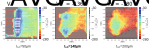
\includegraphics[width=\textwidth]{4_thinning/figures/cartosFautesNew.pdf}
    \caption{Fault susceptibility maps}
    \label{fig:fsm1}
\end{figure}
\begin{figure}[H]
    \centering
    \includegraphics[width=16cm]{4_thinning/figures/cartosFautesSpreading.png}
    \caption{Susceptibility area spreading}
    \label{fig:fsm1spread}
\end{figure}
\begin{figure}[H]
    \centering
    \includegraphics[width=16cm]{4_thinning/figures/cartosCouples.pdf}
    \caption{Fault susceptibility maps couples}
    \label{fig:fsm1couple}
\end{figure}
With geometric and electrical modeling complete, it is now possible to conduct actual experiments in order to verify the meaningfulness of the previous approaches.
In this context, three an STM32F439VIT6 LQFP100 identical targets were thinned to three different levels, from 750 µm to respectively 200 µm, 140 µm and 50 µm, respectively named ST200, ST140 and ST50 for the rest of this Chapter.
In order to verify the three conclusions extracted from the modeling section, three experiments are conducted for each target.

The first experiment aims at measuring the minimal voltage pulse amplitude $V_{PU}^{MIN}$ required to induce a faulty behavior on an IC performing computations.
These experiments are called Fault Susceptibility Maps (FSM).
They allow spotting the region where the IC is sensitive to BBI, no matter which type of induced fault.
Therefore, when mapping an entire IC, it is common to spot various areas not directly involved in the targeted calculation, like the analog voltage regulator or the FLASH memory logic control logic not to cite them all.
As a result, and because in a fault injection context the cryptographic core is very often targeted, it was decided to focus the maps above the STM32 AES core only.
Fig. \ref{fig:fsm1} presents the three performed FSM.
From left to right, $t_{SUB}$ goes from 50 µm, then to 140 µm, finally to 200 µm.
As stated before, the maps are performed above the hardware AES core of the IC, temporally aiming the penultimate AES round.
The scanned area measures 1.7 mm by 1.7 mm, with a displacement step of 40 µm between each point.
$V_{PU}$ was limited to the following range: [30 V ; 280 V], with 5 V steps and a negative polarity.
The pulse width was fixed at 6 ns.
The first important thing to note here is that, as predicted with the geometric and electrical modelings, a thinner substrate allows a lower fault induction threshold.
It is mainly shown thanks to the measurement of the average voltage required to induce a fault across the entire map, annotated at the top of each map.
All of this sustains the first conclusion made in section \ref{chap4:sect:geomModel}.

Then, the second experiment, whose results are shown in Fig. \ref{fig:fsm1spread}, consist in analyzing the spreading of the BBI susceptibility area.
The core of the experiment is identical as before.
However, in order to highlight the spreading effect, it was required to set a lower maximum voltage amplitude (in absolute value).
The value of 180 V was chosen as it is the average voltage of the medium-thinned IC.
What is interesting here is that, for the ST200 target, because the voltage at the epitaxy level cannot reach the threshold value $V_F$ in most cases, the fault area is tiny compared to the other targets, and focused on the AES core.
Then, concerning the ST140 target, thanks to the thinner substrate, the voltage at the epitaxy level can reach a higher value, and thus can cause more logic gates or further logic gates from the probe to have a faulty behavior.
Eventually, the ST50 target shows the largest fault area.
These experiments help to sustain the second conclusion of section \ref{chap4:sect:geomModel}.

Eventually, the last experiment consisted in finding, whenever possible, $(t_{SUB}, V_{PU})$ couples for which the susceptibility area is identical across all targets.
The search for the couples of values was done by first choosing an arbitrary couple for ST200 target, and then calculating the correlation for each couple between the other two susceptibility areas and finding the highest correlation.
Then, to confront the geometric modeling predictions, we calculated, thanks to equation \ref{chap4:sect:geomModel:eqnVpu*}, couples corresponding to

\section{Conclusion \ddc}
In this chapter, I introduced the interest of thinning the substrate of integrated circuits when performing Body Biasing Injection.
In the first place, I presented a geometric approach which allowed me to take a step back from electric simulations.
This approach brought mathematical relations allowing to evaluate preliminary the effects of thinning the substrate of a target IC.
Thanks to this approach, I drew three conclusions on the implications of substrate thinning on \bbi.
Then, thanks to the previous simulation flow introduced in Chapter \ref{chap:3icModeling}, I performed simulations allowing me to complete the geometric approach.
This allowed me to verify the soundness of the geometric conclusions.
After that, I introduced substrate thinning in practice, including a quick look of the tools commonly used.
Eventually, I presented practical experiments on actual thinned ICs, and I was able to verify the soundness of both the geometric and electric approaches.

% !TeX root = ../0_Manuscript.tex

\chapter{Conclusion and perspectives}
\label{chap:6conclusion}
\vspace{-3cm}
\minitoc
\newpage


\section{Contributions}
\label{concl_contrib}

    \subsection{Improvements of existing \bbi platforms}
    Because \bbi was not a very much documented fault injection method before my thesis, the platforms as a whole were not optimized.
    Indeed, most experiments were difficult to reproduce without major variability.
    In addition to this, with our original platform, the range between a normal behavior and a crash of the target was very tight, therefore preventing the execution of fault attacks.
    The goal of circumventing these limitations allowed me to set up enhancements for the practice of \bbi, at the same time efficient and easy to set up.

    \subsection{\bbi simulation flow}
    To better understand the mechanisms at work in integrated circuits under body biasing injection, I developed a simulation flow, allowing me to predict the various disturbances appearing inside the IC targets.
    The base models were extracted from previous works concerning \emfi simulation, and they were enhanced to match the needs of \bbi simulation.
    The models were developed for bulk technologies, considering both \dwF and \twF substrate types.
    However, these models were made to allow for fast simulation of relatively large circuits.
    Therefore, they did not include logic functions.
    To that end, I extended the simulation flow to properly consider logic gates' behavior under \bbi.
    Eventually, these analyses allowed me to understand the mechanisms at work in fault creation under \bbi.

    \subsection{First documented differential fault attack using Giraud's criterion with \bbi}
    Thanks to the platform enhancements, I was able to observe repeatably single bit faults, which are useful when considering constraining fault models.
    Creating single bit faults can be beneficial because they are often used in powerful fault attacks, such as the single bit Giraud's differential fault attack.
    Therefore, by using single bit faults data obtained on my target AES coprocessor, I was able to conduct a Giraud's \dfa and retrieve 14 out of 16 bytes of the secret AES key.

    \subsection{Substrate thinning analysis and \bbi efficiency}
    Similar to what has been done in the past for \lfi \cite{lfiThinning, lfiThinning2}, I conducted similar research on \bbi concerning IC substrate thinning.
    Because the substrate is the physical environment conveying the charge carriers, analyzing what happens, both with electric models and with actual circuits, when the substrate thickness changes, is fundamental.
    I observed that thinning the substrate is mainly useful when the generator power is not sufficient.
    Therefore, while there is enough generator power, increasing the voltage with the substrate thickness leads to very similar results.


\section{Outlooks and discussions}
\label{concl_outlook}
While I have brought new knowledge concerning body biasing injection, there is a lot of room for improvement and for additional work to be done.

First, as I have mentioned in the second chapter, better impedance matching methods can be implemented.
The simplest one is depicted in Fig. \ref{fig:impMatchPhotoNew}.
We started using this implementation in the lab, and it has proven to be more efficient at matching the generator output impedance by providing less ringing and better voltage and pulse width set point values.
Then, to even better provide impedance matching, an active system should be implemented, therefore allowing for adaptability over various pulse generators.

Then, many other aspects can be explored using \bbi.
For instance, RAM fault injection has not yet be studied, and similar to what has been done with \lfi \cite{lfiFaultModel}, memory elements behavior, both static and dynamic, under body biasing injection, could help to have a more profound understanding of the mechanisms at work inside the integrated circuits.
Afterward, FLASH memory modifications, if possible, should be investigated, as if such data modification is possible using \bbi, it could be compelling.

Concerning the modeling of \bbi, especially the simulation follow-up presented in the fourth chapter, more in-depth analysis of more complex logic IC has to be conducted to fully verify the soundness of my conclusions.
For example, and as the substrate simulation is one of the heaviest calculations, computationally speaking, when performing \scs simulation, the two steps simulation flow I presented could be maintained, while simulation an equivalent logical circuit analogous to the \scs one.
However, if by doing so, it eliminates the simultaneous calculation of substrate behavior and logic gates behavior, it still requires a lot of computational power.
Nevertheless, a single \scs simulation data could be used in many logic gates simulations, thus reducing the total computing time.
Eventually, it could be interesting to further explore the geometric approach, especially when considering the various areas of an IC which I did not study, such as the FLASH or the RAM, and analyzing if the geometric approach still makes sense.


\section{Final remarks}
\label{concl_finalremark}
%\vspace{-2cm}
\appendix
\vspace{-1cm}
\UseRawInputEncoding
\lstdefinestyle{mystyle}{
    keywordstyle=\fontfamily{lmss}\color{blue},
    basicstyle=\ttfamily\scriptsize,
    breakatwhitespace=false,
    breaklines=true,
    captionpos=b,
    keepspaces=true,
    numbers=left,
    numbersep=5pt,
    showspaces=false,
    showstringspaces=false,
    showtabs=false,
    tabsize=2
}
\lstset{style=mystyle}
\section*{Standard-cell segment and integrated circuit generation algorithm}
\lstinputlisting[language=Python, caption=\scs generation algorithm Python implementation]{C:/Users/geoff2/Seafile/NETLISTS_SPICE/new/HSPICE GENERATOR v10/hspiceGeneratorV11p1cli.py}


%\nocite{*}
\cleardoublepage
\phantomsection
\addcontentsline{toc}{chapter}{Bibliography}
\mtcaddchapter
\bibliographystyle{unsrt}
\bibliography{references}

\end{document}

